%%%%%%%%%%%%%%%%%%%%%%%%%%%%%%%%%%%%%%%%%%%%%%%%%%%%%%%%%%%%%%%%%%%%%%%%%%%%%%%
%
% IIT Sample THESIS File,   Version 3, Updated by Babak Hamidian on 11/18/2003
%
%%%%%%%%%%%%%%%%%%%%%%%%%%%%%%%%%%%%%%%%%%%%%%%%%%%%%%%%%%%%%%%%%%%%%%%%%%%%%%%
% File: sample3.tex                                   %
% IIT Sample LaTeX File                               %
% by Ozlem Kalinli on 05/30/2003                      %
% Revised by Babak Hamidian on 11/18/2003             %
%%%%%%%%%%%%%%%%%%%%%%%%%%%%%%%%%%%%%%%%%%%%%%%%%%%%%%%
%                                                     %
% This is a sample thesis document created using      %
% iitthesis.cls style file. The PDF output is also    %
% available for your reference. In this file, it has  %
% been illustrated how to make table of contents,     %
% list of tables, list of figures, list of symbols,   %
% bibliography, equations, enumerations, etc.         %
% You can find detailed instructions                  %
% for using the style file in Help.doc,               %
% TableHelp.doc, FigureHelp.doc, and                  %
% Bibliography.doc files.                             %
%                                                     %
%%%%%%%%%%%%%%%%%%%%%%%%%%%%%%%%%%%%%%%%%%%%%%%%%%%%%%%
% Note: The texts that are used in this sample3.tex   %
% file are irrelevant. They are just used to show     %
% you the style created by iitthesis style file.      %
%%%%%%%%%%%%%%%%%%%%%%%%%%%%%%%%%%%%%%%%%%%%%%%%%%%%%%%

\documentclass{iitthesis}

\input .tex
% Document Options:
%
% Note if you want to save paper when printing drafts,
% replace the above line by
%
%   \documentclass[draft]{iitthesis}
%
% See Help file for more about options.

\usepackage[dvips]{graphicx}    % This package is used for Figures
\usepackage{rotating}           % This package is used for landscape mode.
\usepackage{epsfig}
\usepackage{subfigure}          % These two packages, epsfig and subfigure, are used for creating subplots.
% Packages are explained in the Help document.
\usepackage{mathrsfs}
\usepackage{mathptmx}       % selects Times Roman as basic font
\usepackage{helvet}         % selects Helvetica as sans-serif font
\usepackage{courier}        % selects Courier as typewriter font
%\usepackage{type1cm}        % activate if the above 3 fonts are
                            % not available on your system
\usepackage{commath}
\usepackage{makeidx}         % allows index generation
\usepackage{graphicx}        % standard LaTeX graphics tool
                             % when including figure files
\usepackage{multicol}        % used for the two-column index
\usepackage{amsthm}
\usepackage{amsmath}
\usepackage{amsfonts}
\usepackage{amssymb}
\usepackage{color}     % Do not use: colors will appear in gray scale!
\usepackage{url}
\usepackage{verbatim}
\usepackage{cite}
\usepackage{chemarrow}
\usepackage{listings}
 \usepackage{alltt}
 \usepackage{mcode}
%\usepackage[autolinebreaks]{mcode}
\input Ljiangdef.tex
%
%\newcommand{\bbz}{{\bf z}}
%\newcommand{\bbx}{{\bf x}}
%\newcommand{\bby}{{\bf y}}
%\newcommand{\bbX}{{\bf X}}
%\newcommand{\bbY}{{\bf Y}}
%\newcommand{\bbH}{{\bf H}}
%\newcommand{\bbB}{{\bf B}}
%\newcommand{\bbA}{{\bf A}}
%\newcommand{\bbalpha}{\boldsymbol\alpha}
%\newcommand{\bbbeta}{\boldsymbol\beta}
%\newcommand{\bbc}{{\bf c}}
%\newcommand{\bba}{{\bf a}}
%\newcommand{\bbb}{{\bf b}}
%\newcommand{\bbh}{{\bf h}}
%\newcommand{\bbn}{{\bf n}}
%\newcommand{\bbd}{{\bf d}}
%\newcommand{\vgamma}{\boldsymbol\gamma}
%\newcommand{\veczero}{\mathbf{0}}
%\newcommand{\EE}{\mathbb{E}}
%\newcommand{\NN}{\mathbb{N}}
%\newcommand{\DD}{\mathcal {D}}
%\newcommand{\RR}{\mathcal {R}}
%\newcommand{\PP}{\mathcal {P}}
%\newcommand{\HH}{\mathcal {H}}
%\newcommand{\FF}{\mathcal {F}}
%\newcommand{\XX}{\mathcal {X}}
%\newcommand{\QQ}{\mathbb {Q}}
%\newcommand{\FFF}{\mathbb {F}}
%\newcommand{\UU}{\mathbb{U}}
%\newcommand{\Order}{\mathcal O}
%\newcommand{\wup}{{\mathcal U}}
%\newcommand{\ccup}{{\mathcal C}}
%\newcommand{\reals}{\mathbb{R}}
%
%\def\abs#1{\ensuremath{\left \lvert #1 \right \rvert}}
%\newcommand{\ip}[3][{}]{\ensuremath{\left \langle #2, #3 \right \rangle_{#1}}}
%\newcommand{\ch}{\mathcal{H}}
%\newcommand{\fix}{\mathrm{fix}}
%\newcommand{\var}{\mathrm{var}}
%\newcommand{\spann}{\operatorname{span}}
%\newcommand{\eps}{\varepsilon}
%\newcommand{\bx}{{\mathbf x}}
%\newcommand{\by}{{\mathbf y}}
%\newcommand{\bz}{{\mathbf z}}
%\newcommand{\bc}{{\mathbf c}}
%\newcommand{\bv}{{\mathbf v}}
%\newcommand{\ba}{{\mathbf a}}
%\newcommand{\rad}{r^*}
%\newcommand{\XXX}{{\mathfrak X}}
%\newcommand{\rt}{k}
%\newcommand{\E}    {\operatorname{E}}
%\newcommand{\V}    {\operatorname{Var}}
%\newcommand{\err}  {\operatorname{error}}
%\newcommand{\cost} {\operatorname{cost}}
%\newcommand{\id}   {\operatorname{id}}
%\newcommand{\scp}[2]{\langle #1, #2 \rangle}
%
%\DeclareMathOperator{\diag}{diag}
%\DeclareMathOperator{\Trace}{Trace}
%\newtheorem{assump}{Assumption}[chapter]
%\newtheorem{lemma}{Lemma}[chapter]
%\newtheorem{example}{Example}[chapter]
\newtheorem{theorem}{Theorem}[section]
\newtheorem{lemma}[theorem]{Lemma}
\newtheorem{proposition}[theorem]{Proposition}
\newtheorem{corollary}[theorem]{Corollary}
\newtheorem{algorithm}[theorem]{Algorithm}
\newtheorem{defn}{Definition}[theorem]
%\newcommand{\meanMCB}{\tt meanMCBer\_g}
%\newtheorem{corollary}{Corollary}[chapter]
%\newtheorem{definition}{Definition}[chapter]
%\newtheorem{remark}{Remark}[chapter]
%\newtheorem{proof}{Proof}[chapter]
%\renewcommand{\theenumi}{A\arabic{enumi}}

\begin{document}
% Define all the symbols used.

%%% Declarations for Title Page %%%
\title{Guaranteed Adaptive Monte Carlo Methods for Estimating Means of Random Variables}
\author{Lan Jiang}
\degree{Doctor of Philosophy} \dept{Applied Mathematics}
\date{May 2015}
%\copyrightnoticetrue      % crate copyright page or not
%\coadvisortrue           % add co-advisor. activate it by removing % symbol to add co-advisor
\maketitle                % create title and copyright pages


\prelimpages         % Settings of preliminary pages are done with \prelimpages command


%%%  Acknowledgement %%%
\begin{acknowledgement}     % acknowledgement environment, this is optional
\par  This dissertation could not have been written without Dr. Fred
J. Hickernell who not only served as my supervisor but also
encouraged and challenged me throughout my academic program. He and
the other faculty members, Dr. Greg Fasshauer,
Dr. Lulu Kang, guided me through the dissertation process,
never accepting less than my best efforts. I appreciate the joint
work with Dr. Art Owen. I would
also like to thank my husband Xuan Zhou, for his support. I thank them all.
\end{acknowledgement}


% Table of Contents
\tableofcontents
 \clearpage

% List of Tables
\listoftables

\clearpage

%List of Figures
\listoffigures

\clearpage



%%% Abstract %%%
\begin{abstract}           % abstract environment, this is optional
this is abstract
% or \input{abstract.tex}  %you need a separate abstract.tex file to include it.
\end{abstract}
\textpages     % Settings of text-pages are done with \textpages command
% Chapters are created with \Chapter{title} command
\Chapter{INTRODUCTION}\label{introduction}
%Monte Carlo are used to approximate the means, $\mu$, of random variables $Y$, whose distributions are not known explicitly.  The key idea is that the average of a random sample, $Y_1, \ldots, Y_n$, tends to $\mu$ as $n$ tends to infinity. This article explores how one can reliably construct a confidence interval for $\mu$ with a prescribed half-width (or error tolerance) $\varepsilon$.  
%\Chapter{BACKGROUND}

Monte Carlo is a widely used simulation method that can be used to understand and control complex stochastic systems, pricing the financial derivatives, estimating the default probability, evaluating the mean of random variables, perform the numerical integration and solve other real world problems. It is not like the analytical methods, which is limited to simple models whose solution could be solved analytically, nor the numerical methods, which is still limited to certain simple models, Monte Carlo simulation could handle very complex and realistic systems, but we need to do a certain number of replications in order to achieve the desired accuracy.

\Section{Numerical Integration}
Numerical integration covers a board range of algorithms that are used to calculate the numerical value of a definite integral, or estimate the numerical solution of the differential equations.
The basic problem is to calculate the $\mu$ to a certain accuracy, i.e.:
\begin{align}
\mu = \int_a^b f(x)dx \approx \sum_{i=1}^nA_i f(x_i)
\end{align}
where $f(x)$ is the integrad. $x_i$ are the integration points and $A_i$ are the coefficients. The integration points and weights depend on the specific method used and the accuracy required from the approximation.
This problem is often called quadrature. For one dimensional integral, the quadrature method such as trapezoidal rule and Simpson’s rule are known to be efficient if the integrand is smooth. To compute multidimentional integrals, one approach is to phrase the multiple integral as repeated one-dimensional integrals by appealing to Fubini's theorem[cite here]. Cubature[cite here] is one of the well known packages using quadrature methods that work great for low-dimensional integration. However, this approach requires the function evaluations to grow exponentially as the number of dimensions, $d$, increases. This is so called curse of dimensionality[cite here]. One way to overcome this is by Monte Carlo.

\Section{Monte Carlo Simulation} Monte Carlo method is a a scientific computing technique that replies on repeated resampling and statistical analysis to obtain the desired result, it uses some random numbers as a tool to calculate something that is not random. For example, we want to calculate the mean of a random variable $Y$, i.e. $\e(Y) = \mu$ where $\mu$ is a deterministic number.  One way to do it is sampling $n$ independent and identically distributed $X_i$ from the distribution of $X$ and take the average,
$$\mu \approx \hmu_n := \sum_{i=1}^nY_i.$$
The strong law of large numbers states that the sample mean converge to the true mean almost surely, i.e.: $\hmu_n \to \mu$ as $n \to \infty$. Simple Monte Carlo has an error roughly proportional to $1/\sqrt{n}$ for large $n$. The convergence is low comparing to other numerical methods. One way to overcome this is by applying quasi-Monte Carlo techniques, such as using Sobol' or Lattice points[cite here]. They are basically generating low discrepancy sequences in order to get a faster convergence rate. Quasi-Monte Carlo has a rate of convergence close to $O(N^{-1})$, whereas the rate for the Monte Carlo method is $O(N^{-1/2})$.

\Section{Monte Carlo Applications}
Monte Carlo gives a flexible way to approximate the mean $\mu$ of a random variable $Y$, where $\mu=\e(Y)$. One can generate a number of samples $Y_i$ from the distribution of $Y$ and take the sample average as $\hmu_n$, which may be a good estimator of the true mean $\mu$. Some possible real world problems are listed below. 

\Subsection{Option Pricing}
Let $Y$ could be the discount payoff of financial derivatives like options, which depends on the future value of the underlying assets that are driven by some stochastic process like Brownian Motion. one may be interested in the fair price of this option at certain time $t$, this is so called option pricing problem. 

Let $r$ be the interest rate, $T$ be the maturity time, $g(S(t))$ represent the payoff function and $S(t)$  be the stock price dynamic. Then the option price at time 0 is given by $$c=\e[e^{-rT}g(S(T))].$$One simple example is to price the European call option. Let $Y = e^{-rT}(S(T)-K)^+ $, in this way, the fair option price is given by:
$$\mu = \e\left(e^{-rT}(S(T)-K)^+\right)$$
One way to estimate $\mu$ is by sampling a number of $S_i(T)$ and let $Y_i = e^{-rT}(S_i(T)-K)^+$. Then we could estimate $\mu$ by its sample average
$$\hmu_n = \sum_{i=1}^n Y_i = \sum_{i=1}^n( e^{-rT}(S_i(T)-K)^+)$$
The other possible application of Monte Carlo would be the numerical integration via Monte Carlo sampling.

\Subsection{Numerical Integration via Monte Carlo}
Suppose we want to evaluate the multidimensional integral with integrand $f:\reals^d \to \reals$ with respect to some probability density function  $\rho: \reals^d \to [0,\infty)$.
%and some random vector with probability density function $\rho: \reals^d \to [0,\infty)$.
The analytical solution may be written as:
$$\mu = \int_{\reals^d}f(\vx)\rho(\vx)d\vx \quad \text{   where } \vx \in \reals^d \text{ and } \vx \sim \rho(\vx).$$
By appealing Monte Carlo technique, one need to generate a bunch of function values $Y_i$ from the distribution of $\vX$ where $Y_i = f(\vX_i)$, $\vX_i \in \reals^d$. Thus, the true solution could be approximated as
$$\hmu_n = \sum_{i=1}^n f(\vX_i).$$
When $n$ is large enough, $\hmu_n$ may be a good estimator of $\mu$.
%%Suppose we want to calculate the mean of a random variable, whose true mean is unknown, or hard to be calculated analytically. Suppose $Y$ is a random variable, we want to calculate its mean, i.e. $\e(Y) = \mu$, one way to do it is to sample $n$ values of $Y_i$, and let $\hmu_n = \sum_{i=1}^n Y_i$, when $n$ is large enough, $\hmu_n$ may be a good estimator of $\mu$. 

\Subsection{Sample size determination}
How large should $n$ be? One way to determine the sample size $n$ is by Central Limit Theorem(CLT),  which would be explained in Section \ref{clt}. As CLT is an asymptotic results and is true only when $n \to \infty$. We tend to find a finite $n$ in order to make our estimator $\hmu_n$ satisfy the fixed width confidence interval condition 
\begin{align}\label{absCI}
\Pr(\abs{\mu-\hmu_n} \leq \varepsilon_a) \geq 1-\alpha,
\end{align}
where $\varepsilon_a$ is the absolute error tolerance and $\alpha$ is the uncertainty level. 
In Chapter \ref{chapter:meanMCabsg}, under the assumption that the upper bound on the modified kurtosis $\kappa$ is bounded [cite here], i.e.
\begin{align}
\kappa = \frac{\e(Y-\mu)^4}{\sigma^4} \leq \kmax,
\end{align}
we present a two stage algorithm ({\tt meanMCabs\_g}): the first stage generates a conservative upper bound on the variance, and the second stage uses this variance bound and a Berry-Esseen Theorem[cite here], which could be thought as a non-asymptotic CLT, to determine how large $n$ must be for the sample mean to satisfy the fixed width confidence interval condition \eqref{absCI}.

In some practical situations, one may seek to approximate the answer with a certain relative accuracy. e.g. correct to three significant digits. Let $\varepsilon_r$ stands for the relative error tolerance and $\varepsilon_a$ stands for the absolute error tolerance. In this case, one may seek the answer $\hmu_n$ satisfies the following condition:
\begin{align}\label{relCI}
\Pr(\abs{\mu-\hmu_n}\leq \varepsilon_r) \geq 1-\alpha.
\end{align}
This is a global relative error criterion, rather than a point-wise relative error criterion. 
\begin{defn}\label{def:tolfun}
 Define a generalized tolerance function $\tol: [0, \infty) \times [0, \infty) \to [0,\infty)$. Let it be non-decreasing in each of its arguments and satisfy a Lipschitz condition in terms of its second argument, i.e.:
\begin{align}
|\text{tol}(a,b)-\text{tol}(a,b')| \leq |b-b'| \quad \forall a,b,b' \geq 0.
\end{align}
Two examples that one may choose are
\begin{align}
\text{tol}(a,b) = \text{max} (a,b),
\end{align}
\begin{align}
\text{tol}(a,b) = (1- \theta) a + \theta b, \quad 0 \leq \theta \leq 1
\end{align}
\end{defn}By using the hybrid error tolerance function, one may generalize the pure absolute and pure relative error criterion as follows:
\begin{align}\label{hybridCI}
\Pr(\abs{\mu-\hmu_n}\leq \tol(\varepsilon_a, \varepsilon_r\abs{\mu})) \geq 1-\alpha.
\end{align}
In Chapter \ref{chapter:meanMCg}, we proposed an algorithm ({\tt meanMC\_g}) to estimate $\hmu_n$ in order to satisfy the hybrid error condition \eqref{hybridCI}. The procedure is done by bounded the variance from above in the first stage, and loop in the second stage to find the sample size needed in order to reach the stop criteria.

\Section{Fooling functions}
Automatic algorithms commonly determines the computational cost required to approximate the solutions that differ from the true solutions by no more than a given error tolerance, $\varepsilon$. In this way, one require a user specified error tolerance $\varepsilon$ and a black box that generate the function values. Several commonly used software packages have adaptive, automatic algorithms for integrating functions of a single variable, unfortunately, they do not provide any guarantees. On the other hand, most existing guaranteed automatic algorithms are not adaptive, they do not determine the computational cost needed based on the function value sampled. Some examples are
\begin{itemize}
\item {\tt integral} \cite{integralMatlab} in MATLAB, adaptive Gauss-Kronrod quadrature based on {\tt quadva};
\item {\tt chebfun} toolbox [cite here] for MATLAB, which approximates integrals by integrating interrogatory Chebyshev polynomial approximations to the integrads.
\end{itemize}
For these two automatic algorithms, one can easily probe where they sample the integrand, feed the algorithms with zero values and then construct fooling functions for which the automatic algorithms will return zero values for the integral. Figure  [cite] displays these fooling functions for problem $\int_0^1f(x)dx$ for these two algorithms. Each of of these algorithms 
is given the error tolerance $10^{-14}$, unfortunately, the true absolute error is 1. Our critisim is not these algorithms are easily been fooled, instead, our concern is there is no available theory to tell us what is wrong with the integrand when the algorithms are fooled. In this thesis, we plan to address several algorithms that are guaranteed and adaptive for solving Monte Carlo problems.
  \begin{figure}[htbp]
    \centering
    \includegraphics[width=8cm]{chebintbw-2015-08-04-15-30-28.eps} % requires the graphicx package
\includegraphics[width=8cm]{integralbw-2015-08-12-16-01-57.eps} 
    \caption{Plots of the fooling functions,$f$, with $\mu = \int_0^1f(x)dx=1$,bur for which the corresponding algorithms return values of $\hmu=0$}
    \label{fig:ratiovsalpha}
 \end{figure}
 
\Section{Outline of the thesis}
The outline of this thesis is as follows:  Chapter \ref{basicInequalities} provides some basic inequalities and theorems that is related to the algorithms. Chapter \ref{chapter:meanMCabsg} describes an algorithm that is used estimate the mean of a random variable to some absolute error tolerance. A similar but more general algorithm that used to estimate the mean of a random variable to some hybrid error tolerance \ref{def:tolfun} with a high confidence level is described in Chapter \ref{chapter:meanMCg}. Chapter \ref{chapter:cubMCg} focus on numerical integration via Monte Carlo sampling and 
Chapter \ref{chapter:meanMCberg} explains the way to estimate the mean of a Bernoulli random variable to some absolute and relative tolerance with a high confidence level. This thesis ends with a conclusion and some future work.

\Chapter{Basic Theorem and inequalities}\label{basicInequalities}
In Monte Carlo simulation, one want to estimate the mean of a real valued random variable $Y$, usually, it could be written as the expectation form i.e. $\mu:=\e(Y)$. Usually, the random variable $Y$ depends on the some underlying random vector $\vX \in \reals^d$ with probability density function $\rho$, where $Y = f(\vX)$, in other situations, the random vector $\vX$ may have the discrete distribution or may have infinite dimension. Sometimes, the process governing
$Y$ may have a complex form,  i.e. the probability of a bankruptcy, in this case, we may be able to generate the IID sample of $Y$, but may not have a simple formula for computing $\rho$ analytically. 

\Section{Moments}
let $Y$ be a random variable, given the sample size $n$, one generate $Y_1, Y_2, \cdots, Y_n$ samples and calculate the sample mean 
\begin{align}\label{samplemean}
\hmu_n = \sum_{i=1}^n Y_i
\end{align}
and the sample variance
\begin{align}\label{samplevar}
s^2_n = \frac{1}{n-1}\sum_{i=1}^n (Y_i-\hmu_n)^2
\end{align}
as the true mean of $Y$ could be written as the expectation form
\begin{align}\label{truemean}
\mu = \e(Y)
\end{align}
and the true variance is
\begin{align}\label{truevar}
\sigma^2 = \e(Y-\mu)^2
\end{align}
The skewness of $Y$ is defined as 
\begin{align}\label{screwness}
\gamma = \e(Y-\mu)^3/\sigma^3
\end{align}
the modified kurtosis is defined as
\begin{align}\label{kurtosis}
\kappa = \e(Y-\mu)^4/\sigma^4
\end{align}
our main results of this paper relies on the upper bound on the modified kurtosis, which also implies that the variance and skewness are both finite.

\Section{Central Limit Theorem}
The CLT describes how the distribution of $\hmu_n$ approaches a Gaussian distribution as $n \to \infty$.
\begin{theorem}[Central Limit Theorem {\cite[Theorem 21.1]{JP04}}] \label{clt} 
If $Y_1, \ldots, Y_n$ are IID with $\e(Y_i)=\mu$ and $\var(Y_i) = \sigma^2$, then
$$
\frac{\hmu_n-\mu}{\sigma/\sqrt{n}} \to \dnorm(0,1) \quad \text{in distribution, as} \ \ n\to\infty.
$$
\end{theorem}
This theorem implies an approximate confidence interval, called a CLT confidence interval, of the form
\[
\Pr(\abs{\hmu_{n_{\CLT}}-\mu} \le \varepsilon) \approx 1- \alpha \qquad \text{for } n_{\CLT} := \left \lceil \frac{z_{\alpha/2}\sigma^2}{\alpha \varepsilon^2} \right \rceil,
\]
where $z_{\alpha/2}$ is the $1-\alpha/2$ quantile of the standard Gaussian distribution.  When $\sigma^2$ is unknown, it may be replaced by the sample variance $s_n^2$.

\Section{Chebyshev's inequality}
Chebyshev's inequality may be used to construct a fixed-width confidence interval for $\mu$.  It makes relatively mild assumptions on the distribution of the random variable.

\begin{theorem}[Chebyshev's Inequality {\cite[6.1.c]{LB10}}] \label{ChebyThm}If $X$ is a random variable, for any $\varepsilon>0$, $\Pr(\abs{X-E(X)} \ge \varepsilon) \le  \var(X)/\varepsilon^2$.
\end{theorem}
Choosing $X=\sum_{i=1}^n Y_i/n = \mu_n $, noting that $\e(X) = \e(Y) = \mu$, $\var(X) = \var(Y)/n = \sigma^2/n$, and setting $\var(X)/\varepsilon^2=\sigma^2/(n\varepsilon^2) = \alpha$ leads to the fixed-width confidence interval 
\[
\Pr(\abs{\hmu_{n}-\mu} \le \varepsilon) \ge 1- \alpha 
\]
 for 
 \begin{align}
n=N_{\Cheb}(\varepsilon/\sigma,\alpha):= \left \lceil \frac{1}{\alpha (\varepsilon/\sigma)^2} \right \rceil.
 \end{align}
\Section{Cantelli's Inequality}
\begin{theorem}[Cantelli's Inequality {\cite[6.1.e]{LB10}}]\label{CanThm} If $X$ is a random variable with mean $\mu$, and variance $\sigma^2$ then for any $a \geq 0$, it follows that: 
\begin{align}
\Pr(X-\mu \ge a) \le  \frac{\sigma^2}{a^2+\sigma^2}.
\end{align}
\end{theorem}
\Section{Jensen's Inequality}
\begin{theorem}[Jensen's Inequality{\cite[8.4a]{LB10}}]\label{Jensen}
Let$g$ be a convex function on $\reals$. Suppose that the expectations of $X$ and $g(X)$ exist, then
$$g(\e X) \leq \e(g(X)).$$
Equality holds for strictly convex $g$ if and only if $X=EX$ a.s.

\end{theorem}
\Section{The Berry-Esseen Inequality}
\begin{lemma}\label{M3kappalemma}
Let $Y$ be a random variable with mean $\mu$, variance $\sigma^2>0$, third centered moment $M_3 = \e\abs{Y-\mu}^3/\sigma^3 < \infty$ and modified kurtosis $\kappa = \e\abs{Y-\mu}^4/\sigma^4< \infty$, then we have the inequality below:
\begin{align}\label{M3kappa}
M_3\leq \kappa^{3/4}.
\end{align}
\end{lemma}
\begin{proof}
By Jensen's Inequality in Theorem \ref{Jensen}, let the convex function be $g(y) = y^{4/3}$ and define the random variable $X = \abs{Y-\mu}^3$. Then we would have:
$$g(\e X) = \left (\e\abs{Y-\mu}^3\right)^{4/3} \leq \e\left(\left(\abs{Y-\mu}^3\right)^{4/3}\right) = \e(g(X)).$$
which is equivalent to:
$$\frac{\e\left(\abs{Y-\mu}^3\right)}{\sigma^3} \leq \left (\frac{\e\left(\abs{Y-\mu}^4\right)}{\sigma^4}\right)^{3/4}.$$
Then we have:
\begin{align}
M_3\leq \kappa^{3/4}.
\end{align}
\end{proof}
\begin{theorem}[The Berry Esseen Inequality (cite)] \label{BEThm}
Let $Y_1,\cdots,Y_n$ be IID random variables with mean $\mu$, variance $\sigma^2 >0$, and thrid centered moment $M_3 = \e\abs{Y_i-\mu}^3/\sigma^3 < \infty$. Let $\hmu_n = (Y_1+\cdots+Y_n)/n$ denote the sample mean, Then
\[
\abs{\Pr\left(\frac{\hmu-\mu}{\sigma/\sqrt{n}}<x\right)-\Phi(x)} \leq \delta_n(x,M_3):=\frac{1}{n}\min\left( A_1(M_3+A_2),  A_3(M_3+A_4), A_5M_3, \frac{A_6M_3}{1+\abs{x}^3}\right)
\]
where $A_1 = 0.3322$, $A_2 = 0.429$, $A_3=0.3031$, $A_4=0.646$, $A_5=0.469$ and $A_6=18.1139$.
\end{theorem}
By applying theorem \ref{BEThm} with given $M_3$, let $\hmu_n$ donates a sample mean of $n$ IID random instances of $Y$, then the non-uniform Berry-Esseen inequality implies that
\begin{align} 
&\Prob\left[\abs{\mu-\hmu_n}  \le \varepsilon \right]\nonumber\\
&=\Prob\left[\frac{\hmu_n - \mu}{\sigma/\sqrt{n}} \le \frac{\sqrt{n}\varepsilon}{\sigma} \right]-\Prob\left[\frac{\hmu_n - \mu}{\sigma/\sqrt{n}} < -\frac{\sqrt{n}\varepsilon}{\sigma}\right] \nonumber \\ 
&\ge \left[\Phi(\sqrt{n}\varepsilon/\sigma)-\delta_n(\sqrt{n}\varepsilon/\sigma,M_3)\right] -\left[\Phi(-\sqrt{n}\varepsilon/\sigma) + \delta_n(-\sqrt{n}\varepsilon/\sigma,M_3)\right] \nonumber \\
&=1-2[\Phi(-\sqrt{n}\varepsilon/\sigma) + \delta_n(\sqrt{n}\varepsilon/\sigma,M_3)] =: g(n, \sigma, M_3, \varepsilon), \label{BEresult}
\end{align}
since $\delta_n(-x,M_3)=\delta_n(x,M_3)$.  The probability of
making an error no greater than $\varepsilon$ is bounded below by $1-\alpha$, i.e., the fixed width confidence interval \eqref{absCI} holds with $\hmu=\hmu_n$, provided $n \ge N_{\text{BE}}(\varepsilon,\sigma,\alpha,M_3)$, where the Berry-Esseen sample size is
\begin{equation}\label{BEn}
N_{\text{BE}}(\varepsilon/\sigma,\alpha,M_3) := \min  \left \{ n \in \naturals : \Phi\left(-\sqrt{n}\varepsilon/\sigma  \right)+\Delta_n(\sqrt{n}\varepsilon/\sigma,M_3)
\le \frac{\alpha}{2} \right \}.
\end{equation}
To compute $N_{\text{BE}}(\varepsilon/\sigma,\alpha,M_3)$, we need to know
$M_3$. In practice, substituting an upper bound on $M_3$ yields an upper bound on the necessary sample size.
As $M_3 \leq \kappa^{3/4}$ by Lemma \ref{M3kappalemma}, the sample size calculated by \eqref{BEn} is also $N_{\BE}\left(\varepsilon/\sigma,\alpha,\kappa^{3/4}\right) $.
%As the condition of the 
%Define the sample sized calculated by Chebyshev's inequality and Berry-Esseen inequality as:
%\begin{align*}
%N_{CB} (\varepsilon_a/\hsigma,\alpha_{\mu}, \kmax^{3/4}) = \min \left\{N_{\BE}, N_{\Cheb}\right\}
%\end{align*}

\Section{Hoeffding's Inequality}
The conservative fixed-width confidence interval for general random variables constructed by  \cite{HJLO12} uses the Berry-Esseen Inequality \cite[Section 4.1]{LB10} and Cantelli's Inequality \cite[Section 6.1]{LB10}. However, in view of the particular form of the Bernoulli distribution, we may rely on inequalities that assume some bound on the random variable.  Here we use Hoeffding's Inequality \cite{H63}, which seems more suitable than, say, the Chernoff bound \cite{chernoff52}.  Below is the a special case of Hoeffding's Inequality for random variables lying in $[0,1]$.
\begin{theorem}[Hoeffding's Inequality {\cite{H63}}] \label{hoeff}
If $Y_1$, $Y_2$, $\cdots$, $Y_n$ are IID observations such that $\e(Y_i)=p$ and $0 \leq Y_i \leq 1$, define $\hp_n=\sum_{i=1}^n Y_i/n$. Then, for any $\varepsilon>0$, 
$$\Pr(\hp_n-p \geq \varepsilon) \leq e^{-2n\varepsilon^2},$$
$$\Pr(p-\hp_n \geq \varepsilon) \leq e^{-2n\varepsilon^2},$$
$$\Pr(\abs{\hp_n-p} \geq \varepsilon) \leq 2e^{-2n\varepsilon^2}.$$
\end{theorem}

\Section{Fr\'{e}chet formula}
\begin{theorem}[Fr\'{e}chet Formula] \cite{FrechetIneq}
Probability of a logical conjunction have the following inequality:
\begin{align}
\max(0, P(A_1) + P(A_2)+\cdots +P(A_n)-(n -1)) \leq P\left(\bigcap_{i=1}^n A_i\right)\leq \min(P(A_1), P(A_2), ..., P(A_n))
\end{align}
\end{theorem}
\begin{lemma}\cite[Lemma 1]{HJLO12} \label{samplevarbound}
Let $Y_1,\cdots,Y_n$ be IID random variables with variance $\sigma^2>0$ and modified kurtosis $\kappa$, Let $s_n^2$ be the sample variance defined at \eqref{samplevar}. Then
\begin{subequations}
\begin{gather}
\Pr\left( s_n^2 < \sigma^2 \left (1+\sqrt{\left (\kappa-\frac{n-3}{n-1}\right)\left (\frac{1-\alpha}{\alpha n}\right )}\right)\right) \geq 1-\alpha,\label{boundsamplevar1}\\ 
\Pr\left( s_n^2 >\sigma^2 \left (1-\sqrt{\left (\kappa-\frac{n-3}{n-1}\right)\left (\frac{1-\alpha}{\alpha n}\right )}\right)\right) \geq 1-\alpha.\label{boundsamplevar2}
\end{gather}
\end{subequations}

\end{lemma}
%this is the lemma to bound the \hsigma from above
\begin{lemma}\label{lowerboundhsigma}
By the same assumption in Lemma \ref{samplevarbound}. Define an upper bound on variance estimation as $\hsigma^2 = \fudge^2 s_{n_{\sigma}}^2$, where $\fudge^2$ is the variance inflation factor. If $\kappa \leq \kmax$, where $\kmax$ is defined in \eqref{kappamaxdef}, then $$\Pr (\hsigma^2 > \sigma^2)\geq 1-\alpha_{\sigma}$$
\end{lemma}
\begin{proof}
Applying the inequality \eqref{boundsamplevar2} in Lemma \ref{samplevarbound}, since the assumption is $\kappa \leq \kmax$, then we have the following inequality: 
\begin{align*}
1-\alpha_{\sigma} &\geq \Pr\left( s_{n_{\sigma}}^2 > \sigma^2 \left (1-\sqrt{\left (\kappa-\frac{n_{\sigma}-3}{n_{\sigma}-1}\right)\left (\frac{1-\alpha_{\sigma}}{\alpha_{\sigma} n_{\sigma}}\right )}\right)\right)\\&
 \geq  Pr\left( s_{n_{\sigma}}^2 > \sigma^2 \left (1-\sqrt{\left (\kmax -\frac{n_{\sigma}-3}{n_{\sigma}-1}\right)\left (\frac{1-\alpha_{\sigma}}{\alpha n_{\sigma}}\right )}\right)\right).
 \intertext{Plugging in $\kmax$ defined in \eqref{kappamaxdef} would yield:}
 1-\alpha_{\sigma} 
 &\geq \Pr\left( s_{n_{\sigma}}^2 > \sigma^2 \left (1-(1-1/\fudge^2)\right) \right)\\&
 =\Pr(\fudge^2s_{n_{\sigma}}^2  > \sigma^2 )\\
 & = \Pr(\hsigma^2  > \sigma^2 )
\end{align*}
This inequality explains that if the modified kurtosis $\kappa$ is bounded by $\kmax$, then the variance $\sigma^2$ would have a probabilistic upper bound $\hsigma^2$ with confidence level $1-\alpha_{\sigma}$.
\end{proof}

\begin{lemma}\label{upperboundhsigma}
Apply the result in Lemma \ref{lowerboundhsigma} and define the upper bound on $\hsigma^2$ as:
\begin{align}\label{sigup}
\hsigma_{\up}^2 (\beta) := \left(\fudge^2+(\fudge^2-1)\sqrt{\frac{\alpha_{\sigma}(1-\beta)}{(1-\alpha_{\sigma})\beta}}\right)\sigma^2.
\end{align}
Then the following inequality would be true: 
\begin{align}\label{hsighsigupineq}
\Pr(\hsigma^2 <\hsigma_{\up}^2) \geq 1-\beta.
\end{align}
\end{lemma}

\begin{proof}
Apply the inequality \eqref{boundsamplevar1} in lemma \ref{samplevarbound}, multiply both side of the inequality by the fudge factor $\fudge$. As we assume $\kappa \leq \kmax$,  replacing the modified kurtosis $\kappa$ by $\kmax$ would yield:
\begin{align*}
1-\beta &\leq Pr\left( s_n^2 < \sigma^2 \left (1+\sqrt{\left (\kappa-\frac{n_{\sigma}-3}{n_{\sigma}-1}\right)\left (\frac{1-\beta}{\beta n_{\sigma}}\right )}\right)\right)\\&
 = Pr\left( \fudge^2 s_n^2 < \fudge^2 \sigma^2 \left (1+\sqrt{\left (\kappa-\frac{n_{\sigma}-3}{n_{\sigma}-1}\right)\left (\frac{1-\beta}{\beta n_{\sigma}}\right )}\right)\right)\\&
 \leq Pr\left( \hsigma^2 < \fudge^2 \sigma^2 \left (1+\sqrt{\left (\kmax-\frac{n_{\sigma}-3}{n_{\sigma}-1}\right)\left (\frac{1-\beta}{\beta n_{\sigma}}\right )}\right)\right).\\&
\nonumber
&  \intertext{Plugging in the $\kmax$ defined in \eqref{kappamaxdef}, and $\hsigma_{\up}$ defined in \eqref{sigup} would yield:}\\
&1-\beta \\
&\leq Pr\left( \hsigma^2 < \fudge^2 \sigma^2 \left (1+\sqrt{\left (\frac{n_{\sigma}-3}{n_{\sigma}-1} + \left(\frac{ \alpha n_{\sigma}}{1-\alpha}\right) \left(1 - \frac{1}{\fudge^2}\right)^2- \frac{n_{\sigma}-3}{n_{\sigma}-1}\right)\left (\frac{1-\beta}{\beta n_{\sigma}}\right )}\right)\right)\\
& = Pr\left( \hsigma^2 < \sigma^2 \left(\fudge^2+(\fudge^2-1)\sqrt{\frac{\alpha(1-\beta)}{(1-\alpha)\beta}}\right)\right)\\
& =\Pr \left ( \hsigma^2< \hsigma_{\up}^2 \right)
\end{align*}
\end{proof}

\Chapter{Guaranteed Monte Carlo method with an absolute error tolerance}\label{chapter:meanMCabsg}
Here, we would illustrate our two-stage algorithm. In the first stage, we sample $n_\sigma$ IID samples from the distribution of $Y$, from this sample we compute the sample variance, $s_{n_\sigma}^2$, according to \eqref{samplevar} and estimate the upper bound on variance $Y_i$ by $\hsigma^2 = \fudge^2s_{n_{\sigma}}^2$, where $\fudge^2>1$ is a variance inflation factor. For the second stage, we replace the true variance $\sigma^2$ by its upper bound $\hsigma^2$, then use the Berry-Esseen Theorem \ref{BEThm} to get the sample size needed for computing the sample mean $\hmu$, if the modified kurtosis $\kappa$ is less than $\kmax$, then we could guarantee that the fixed width confidence interval condition \eqref{absCI} may be satisfied.

\Section{the Algorithm :{\tt meanMCabs\_g}} 
Before illustrating the algorithm, we define some parameters. Given the uncertainty $\alpha_{\sigma}$, the sample size $n_{\sigma}$ and the fudge factor, define
\begin{equation}
\label{kappamaxdef}
\kappa_{\max} (\alpha_\sigma, n_{\sigma},\fudge):= \frac{n_{\sigma}-3}{n_{\sigma}-1} + \left(\frac{ \alpha_\sigma n_{\sigma}}{1-\alpha_\sigma}\right) \left(1 - \frac{1}{\fudge^2}\right)^2.
\end{equation}
Next, define the sample size calculated by CLT as:
\begin{equation}\label{NCLT}
N_{\mathrm{CLT}}(\varepsilon/\sigma,\alpha)
= 
\Bigl\lceil
\Bigl(
\frac{z_{\alpha/2}\sigma}{\varepsilon}
\Bigr)^2
\Bigr\rceil
\end{equation}
and the sample size calculated by Chebyshev's inequality as:
\begin{equation}\label{NCheby}
N_{\text{Cheb}}(\varepsilon/\sigma,\alpha)
= 
\Bigl\lceil\frac{\sigma^2}{\alpha\varepsilon^2}\Bigr\rceil
\end{equation}
By applying theorem \ref{BEThm}, we could get the sample size calculated by Berry Esseen inequality as:
\begin{equation}\label{NBE}
N_{\text{BE}}(\varepsilon/\sigma,\alpha,M_3) := \min \left \{ n \in \naturals : \Phi\left(-\sqrt{n}\varepsilon/\sigma  \right)+\delta_n(\sqrt{n}\varepsilon/\sigma,M_3)
\le \frac{\alpha}{2} \right \}.
\end{equation}
As our assumption is $\kappa \leq \kmax$, applying \eqref{M3kappa} yields 
\begin{align}\label{M3kmax}
M_3 \leq \kmax^{3/4}.
\end{align}
Thus, we could define the sample size obtained by both Chebyshev and Berry Esseen inequality as:
\begin{align}\label{NCB}
N_{CB} (\varepsilon/\sigma,\alpha, \kmax^{3/4})  = \min \left \{ N_{\Cheb}\left(\varepsilon/\sigma,\alpha\right),N_{\BE}\left(\varepsilon/\sigma,\alpha, \kmax^{3/4}\right)\right \}.
\end{align}
In details, the two-stage algorithm works as described below:
\begin{algorithm}[{\tt meanMCabs\_g}]\label{alg:meanMCabsg}
Given a random number generator $Y$ and the absolute error tolerance $\varepsilon_a$, one specifies the following parameters:
\begin{itemize}
\item the absolute error tolerance $\varepsilon_a >0$,
\item the uncertainty level $\alpha \in (0,1)$,
\item the uncertainty level for variance estimation $\alpha_\sigma \in (0,\alpha)$,
\item the sample size used to estimate the variance, $n_{\sigma} \in \naturals$, $n_{\sigma} \geq 2$,
\item the variance inflation factor $\fudge^2 >1$.
%\item the kurtosis max $\kmax(n_\sigma,\alpha_\sigma,\fudge)$ as defined in xxxxx.
\end{itemize}
With the given parameters, first calculate $\kmax=\kappa_{\max}(n_\sigma,\alpha_\sigma,\fudge)$ as defined in \eqref{kappamaxdef}, then do the following:
\begin{enumerate}
%\renewcommand{\labelenumi}{\alph{enumi})}
\item Compute the sample variance, $s^2_{n_{\sigma}}$, using a simple random sample of size $n_\sigma$. Let $\hsigma^2 = \fudge^2 s^2_{n_\sigma}$ be the upper bound on variance.
\item Compute the uncertainty for the second stage $\alpha_\mu = 1-(1-\alpha)/(1-\alpha_{\sigma})$ and the sample size for the mean estimation,
\begin{align}\label{NCBmeanMCabs}
n_\mu = N_{CB} (\varepsilon_a/\hsigma,\alpha_\mu, \kmax^{3/4}).
\end{align}
Sample $n_\mu$ IID samples from the distribution of $Y$ that are interdependent of those used to estimate $\sigma^2$. Calculate the mean $\tmu$,
\begin{align}\label{hmun}
\tmu = \frac{1}{n_\mu}\sum_{i = n_\sigma+1}^{n_\sigma+n_\mu}Y_i.
\end{align}
\end{enumerate}
\end{algorithm}
The success of the Algorithm \ref{alg:meanMCabsg} is proved in the following theorem.
\begin{theorem}\label{thm:meanMCabsg}
Let $Y$ be a random variable with mean $\mu$, variance $\sigma^2 >0$, and modified kurtosis $\kappa$. Let $\kmax=\kmax(n_\sigma,\alpha_\sigma,\fudge)$ be as defined in \eqref{kappamaxdef}. For any random variable $Y$ lying in the cone of functions with bounded kurtosis, $\cc_{\kappa_{\max}}$, i.e.
$\kappa\leq\kmax(\alpha_{\sigma},n_{\sigma},\fudge)$, Algorithm \ref{alg:meanMCabsg} above yields an estimate $\tmu$ given by \eqref{hmun} that satisfies the fixed width confidence interval condition
\begin{align}
\Pr\left( \abs{\mu-\tmu} \leq \varepsilon_a \right) \geq 1-\alpha.
\end{align}
\end{theorem}
\begin{proof}
Let $\varepsilon_a$, $\alpha_\sigma$, $n_\sigma$, $\fudge$ be the parameters and $\hsigma^2$ be a random variable depending on the random samples $Y_i$, $i = 1,2,\cdots, n_{\sigma}$ as given in Algorithm \ref{alg:meanMCabsg}. By Lemma \ref{lowerboundhsigma}, if the modified kurtosis $\kappa \leq \kmax(\alpha_{\sigma},n_{\sigma},\fudge)$, then we could find a probabilistic upper bound on $\sigma^2$, which is:
$$\Pr (\hsigma^2 > \sigma^2)\geq 1-\alpha_{\sigma}.$$
Since $\hsigma$ is random, $n_\mu$ as defined in \eqref{NCBmeanMCabs} is also random. Thus, the randomness of $\tmu$ comes both from the sample size $n_\mu$ and the random number generator $Y$. By adding the extra condition inside the probability, we have the inequality below:
\begin{align*}
&\Pr(\abs{\mu-\tmu} \leq \varepsilon_a) \geq  \Pr({\abs{\mu-\tmu} \leq \varepsilon_a}, {\hsigma >\sigma})
= \Pr(\abs{\mu-\tmu} \leq \varepsilon_a |\hsigma>\sigma)\Pr(\hsigma >\sigma)\\&\geq \Pr(\abs{\mu-\tmu} \leq \varepsilon_a |\hsigma > \sigma)(1-\alpha_\sigma).
\intertext{As the sample $n\_\mu$ used to calculate $\tmu$ is defined by Berry Esseen inequality in \eqref{NCBmeanMCabs}, we have:}
&\Pr(\abs{\mu-\tmu} \leq \varepsilon_a) \\
& \geq \Pr\left( \left({\abs{\mu-\sum_{i=1}^{n_\mu} Y_i} \leq \varepsilon_a},{n_\mu= N_{CB}\left(\varepsilon_a/\hsigma,\alpha_\mu, \kmax^{3/4}\right)}\right){1_{\hsigma >\sigma}}\,\bigg\vert \,\hsigma>\sigma\right)\left(1-\alpha_\sigma\right).
\intertext{Given $\hsigma >\sigma$, $\kappa \leq \kmax$, by applying Berry Esseen inequality we have:}
&\Pr(\abs{\mu-\tmu} \leq \varepsilon_a) \geq g\left(n_\mu,\hsigma, \kmax^{3/4}, \varepsilon\right)\left(1-\alpha_\sigma\right) = (1-\alpha_\mu)(1-\alpha_\sigma) = (1-\alpha).
\end{align*}
\end{proof}

\Section{The upper bound on cost of the Algorithm {\tt meanMCabs\_g}}
The cost of the Algorithm \ref{alg:meanMCabsg} is determined by two part: the sample size $n_{\sigma}$ used to estimate the variance $\sigma$ in stage one, and the sample size $n_\mu$ used to estimate the mean $\mu$ in stage two, thus, the total cost is 
$$n_{\rm tot} = n_\sigma+n_\mu.$$
Although the $n_\sigma$ is deterministic, $n_\mu$ is a random variable. The cost of Algorithm \ref{alg:meanMCabsg} may be defined probabilistically. 
\begin{theorem}
The two stage Monte Carlo algorithm for fixed width confidence intervals based on IID sampling described in Algorithm \ref{alg:meanMCabsg} has a probabilistic cost bound $n_{\up} =n_\sigma+\bar{n}_{\mu}$ where $\bar{n}_{\mu}=N_{CB}\left(\varepsilon_a/\hsigma_{\up},\alpha_\mu, \kmax^{3/4}\right)$.
\begin{align}
\Pr \left(n_{\tot} < n_{\up}\right)  \geq 1-\beta.
\end{align}
\end{theorem}

\begin{proof}
As the only random quantity in $n_\mu$ is $\hsigma^2$, we need to bound $\hsigma^2$ so as  to bound $n_{\mu}$.
 By applying the definition of $\hsigma_{\up}^2$ in Lemma \ref{upperboundhsigma} and letting $\bar{n}_{\mu} = N_{CB}\left(\varepsilon_a/\hsigma_{\up},\alpha_\mu, \kmax^{3/4}\right)$, we would have:
\begin{align}
& \Pr(n_{\mu} < \bar{n}_{\mu})  = \Pr\left (N_{CB}\left(\varepsilon_a/\hsigma,\alpha_\mu, \kmax^{3/4}\right) < N_{CB}\left(\varepsilon_a/\hsigma_{\up},\alpha_\mu, \kmax^{3/4}\right) \right)\\&
 = \Pr \left(\hsigma^2 < \hsigma_{\up}^2 \right) \geq 1-\beta
\end{align}
Let $n_{\up} =n_\sigma+\bar{n}_{\mu} $
which means:
\begin{align}
\Pr \left(n_{\tot} < n_{\up}\right)  \geq 1-\beta.
\end{align}
\end{proof}
\Section{Numerical integration via Monte Carlo sampling}
An important special case of computing $\mu =\e(Y)$ is when $Y = f(\vX)$ for some function $f:\reals^d \to \reals$ and some random vector $\vX$ with probability density function $\rho: \reals^d \to [0,\infty)$. One may then interpret the mean of $Y$ as the multidimensional integral
\begin{align*}
\mu = \mu(f) = \e(\vY) = \int_{\reals^d}f(\vx)\rho(\vx)d\vx.
\end{align*}
Note that given the problem of evaluating $\mu = \int_{\reals^d}g(\vx)d\vx$, one must choose a probability density function $\rho$ for which one can easily generate random vectors $\vX$, then set $f = g/\rho$. The quantities $\sigma^2$ and $\kappa$ defined above can be written in terms of weighted $\mathcal{L}_p$ norms of $f$:
\begin{align}
\norm{f}_p:=\left\{ \int_{\reals^d}\abs{f(\vx)}^p\rho(\vx)d\vx\right\}^{1/p}, \quad \sigma^2 = \norm{f-\mu}_2^2,\quad \kappa = \frac{\norm{f-\mu}_4^4}{\norm{f-\mu}_2^4}.
\end{align}
For a given $g$, the choice of $\rho$ is not unique, and making an optimal choice belongs to the realm of the importance sampling. The assumption of bounded kurtosis, [refer here] required by Algorithm \ref{alg:meanMCabsg}, corresponds to an assumption that integrand $f$ lies in the cone of functions[cite yuhan hickernell paper].
\begin{align}
C_{\kmax} = \left\{ f \in \mathcal{L}_4: \norm{f-\mu(f)}_4 \leq \kmax^{1/4} \norm{f-\mu(f)}_2\right\}.
\end{align}
This is in contrast to a ball of functions, which wound be the case if one was satisfying a bounded variance conditions.
Below, we will present our Algorithm {\tt cubMCabs\_g} to evaluate the integration
$$\mu = \int_{\reals^d} f(\vx)\rho(\vx)d\vx, \quad \text{where}\quad \vx \in \reals^d \quad \text{and}\quad  \vx \sim \rho(\vx)$$
to some specified absolute error tolerance $\varepsilon_a$.
%Then Algorithm {\tt meanMC\_g} is the one that can be used to estimate the mean of random variable $Y$. Let $\vY = f(\vX)$ where $X$ is a random $d$-vector with probability density function $\rho$, then $\mu$ could be interpreted as the integral $\int_{\reals^d}f(\vx)\rho(\vx)d\vx$, and the Monte Carlo method could be used to estimate a multidimensional cubature.
\Section{The Algorithm {\tt cubMCabs\_g }}
\begin{algorithm}\label{alg:cubMCabsg} 
User specifies the following parameters defining the algorithm:
\begin{itemize}
\item the integrand $f(\vx)$,
\item the integration interval $[a_i,b_i]^d$,
\item the probability density function $\rho(\vx)$,
\item the absolute error tolerance $\varepsilon_a \geq 0$,
\item uncertainty level for the confidence interval, $\alpha\in (0,1)$,
\item the uncertainty level for variance estimation $\alpha_\sigma \in (0,\alpha)$,
\item variance inflation factor, $\fudge \in (1,\infty)$, 
\item initial sample size for variance estimation, $n_{\sigma} \in \naturals$, $n_{\sigma} \geq 2$.
\end{itemize} 
With the given parameters, first calculate $\kmax=\kappa_{\max}(n_\sigma,\alpha_\sigma,\fudge)$ as defined in \eqref{kappamaxdef}, then do the following:
\begin{enumerate}
%\renewcommand{\labelenumi}{\alph{enumi})}
\item In the first stage, sample $n_\sigma$ values of random vector $\vX_i$ from the distribution of $\vX$ with probability density function $\rho(\vX)$ and obtain $n_\sigma$ function values of $f(\vX_i)$. Use this to calculate the sample mean $$\hat{I}_{n_\sigma} = \frac{1}{n_\sigma}\sum_{i=1}^{n_\sigma} f(\vX_i),$$ and sample variance $$s_{n\sigma}^2 = \frac{1}{n_\sigma-1}\sum_{i=1}^{n\sigma} (f(\vX_i)-\hat{I}_{n_\sigma})^2.$$ Also approximate the upper bound on variance by $\hsigma^2 = \fudge^2 s^2_{n_\sigma}$. 

\item After the preparation of the upper bound on variance, compute the uncertainty level for the second stage $\alpha_\mu = 1-(1-\alpha)/(1-\alpha_{\sigma})$ and the sample size for the mean estimation,
\begin{align}\label{NCBmeanMCabs}
n_\mu = N_{CB} (\varepsilon_a/\hsigma,\alpha_\mu, \kmax^{3/4}).
\end{align}
Sample $n_\mu$ values of random vector $\vX_i$ that are interdependent of those used to calculate $\hsigma^2$ from the distribution of $\vX$ with probability density function $\rho(\vX)$, then calculate the $n_\mu$ function values of $f(\vX_i)$. Use this to calculate the sample mean 
\begin{align}\label{hmun}
\hat{I}= \frac{1}{n_\mu}\sum_{i = n_\sigma+1}^{n_\sigma+n_\mu}f(\vX_i).
\end{align}
\end{enumerate}
\end{algorithm}

\Section{Numerical example of {\tt cubMCabs\_g}}

\Subsection{Integrating a single hump}\label{subsec:meanmcabssinglehump}
Accuracy and timing results have been recorded for the integration problem $\mu=\int_{[0,1]^d} f(\vx) \, \dif \vx$ for a single hump test integrand
\begin{equation} \label{GaussianTestFun}
f(\vx)=a_0 + b_0\prod_{j=1}^d\left[ 1 +b_j \exp \left(-\frac{(x_j-h_j)^2}{c_j^2}\right) \right].
\end{equation}
Here $\vx$ is a $d$ dimensional vector, and $a_0, b_0, \ldots, b_d, c_1, \ldots, c_d, h_1, \ldots, h_d$ are parameters. Figure \ref{fig:GaussianTestFun} shows the results of different algorithms being used to integrate $500$ different instances of $f$.  For each instance of $f$, the parameters are chosen as follows:
\begin{itemize} 
\item $b_1, \ldots, b_d \in [0.1,10]$ with $\log(b_j)$ being i.i.d.\ uniform,
\item $c_1, \ldots, c_d \in [10^{-6},1]$ with $\log(c_j)$ being i.i.d.\ uniform,
\item $h_1, \ldots, h_d \in [0,1]$ with $h_j$ being i.i.d.\ uniform,
\item $b_0$ chosen in terms of the $b_1, \ldots, b_d, c_1, \ldots, c_d, h_1, \ldots, h_d$ to make $\sigma^2 =\norm[2]{f-\mu}^2 \in [10^{-2}, 10^2]$, with $\log(\sigma)$ being i.i.d.\ uniform for each instance, and
\item $a_0$ chosen in terms of the $b_0, \ldots, b_d, c_1, \ldots, c_d, h_1, \ldots, h_d$ to make $\mu=1$.
\end{itemize}
These ranges of parameters are chosen so that the algorithms being tested fail to meet the error tolerance a significant number of times.
\begin{figure}
\centering
\begin{minipage}{7cm} \centering \includegraphics[width=7cm]
{gaussiand=1iidErrTime-2015-08-12-16-25-16.eps} \\ {\tt cubMCabs\_g}  \end{minipage}
\begin{minipage}{7cm} \centering \includegraphics[width=7cm]{gaussiand=1cubSobolErrTime-2015-08-12-16-25-17.eps} \\  {\tt cubSobol\_g}\end{minipage}
\begin{minipage}{7cm} \centering \includegraphics[width=7cm]{gaussiand=1cubLatticeErrTime-2015-08-12-16-25-17.eps} \\ {\tt cubLattice\_g} \end{minipage}
\begin{minipage}{7cm} \centering \includegraphics[width=7cm]
{gaussiand=1chebfunErrTime-2015-08-12-16-25-18.eps} \\ {\tt chebfun} \end{minipage}
\begin{minipage}{7cm} \centering \includegraphics[width=7cm]
{gaussiand=1integralErrTime-2015-08-12-16-25-18.eps} \\ {\tt integral} \end{minipage}
\caption{Execution times and errors for the single hump test function \eqref{GaussianTestFun} for $d=1$ and error tolerance $\varepsilon_a=10^{-3}$, and a variety of parameters giving a range of $\sigma$ and $\kappa$. Those points to the left/right of the dashed vertical line represent successes/failures of the automatic algorithms.  The solid line shows that cumulative distribution of actual errors, and the dot-dashed line shows the cumulative distribution of execution times.  For the Algorithm \ref{cubMCabsg} the points labeled * are those for which the Corollary \ref{thm:meanMCabsg} guarantees the error tolerance.\label{fig:GaussianTestFun} }
\end{figure}

These $500$ random constructions of $f$ with $d=1$ are integrated using {\tt integral},  {\tt cubMCabs\_g}, {\tt chebfun}, and {\tt cubLattice\_g}, {\tt cubSobol\_g} [cite here], 
%The sample size is increased until this error estimate decreases to no more than the tolerance
%and an automatic quasi-Monte Carlo algorithm that uses scrambled Sobol' sampling \citep{Owe95,Owe96,Owe97,Mat98,HonHic00a,DicPil10a}.  For the Sobol' sampling algorithm the error is estimated by an inflation factor of $1.1$ times the sample standard deviation of $8$ internal replicates of one scrambled Sobol' sequence \citep{Owe06a}.  The sample size is increased until this error estimate decreases to no more than the tolerance.  We 
%have not yet found simple conditions on integrands for which this procedure is guaranteed to produce an estimate satisfying the error tolerance, 
%and so we do not discuss it in detail.  We are however, intrigued by the fact that it does seem to perform rather well in practice.
%
For all but {\tt chebfun}, the specified absolute error tolerance is $\epsilon=10^{-3}$.  The algorithm {\tt chebfun} attempts to do all calculations to near machine precision.  The observed error and execution times are plotted in Figure \ref{fig:GaussianTestFun}.  Whereas {\tt chebfun} uses a minimum of $2^3+1=9$ function values, {\tt cubMCabs\_g}  takes $\alpha=0.01$, and $\fudge=1.2$.  For the plot on the left, $n_\sigma=2^{13}=8192$, which corresponds to  $\kmax=4.84$. 
%
Figure \ref{fig:GaussianTestFun} shows that {\tt integral} is quite fast, nearly always providing an answer in less than $0.01$ seconds.  Unfortunately, it successfully meet the error tolerance only about $18\%$ of the time.  The difficult cases are those where $c_1$ is quite small, and these algorithms miss the sharp peak.  The performance of {\tt chebfun} is similar to that of {\tt integral}. {\tt chebfun} plots there are a significant proportion of the data that do not appear because their errors are smaller than $10^{-5}$.
%
In the plots for {\tt cubMCabs\_g}, an asterisk is used to label those points satisfying $\kappa \le \kmax$, where $\kappa$ is defined in \eqref{kurtosis}. All such points fall within the prescribed error tolerance,
which is even better than the guaranteed confidence of $99\%$.  Those points labeled with a dot, are those for which $\kappa > \kmax$, and so no guarantee holds. The points labeled with a diamond are those for which  {\tt cubMCabs\_g}  attempts to exceed the cost budget that we set, i.e., it wants to choose $n_\mu$ such that $n_{\sigma}+n_\mu > N_{\max}:=10^9$. In these cases $n_\mu$ is chosen as $\lfloor 10^9 - n_\sigma \rfloor$, which often is still large enough to get an answer that satisfies the error tolerance. 

 {\tt cubMCabs\_g}  performs somewhat more robustly than {\tt integral}, {\tt chebfun}, because it requires only a low degree of smoothness and takes a fairly large minimum sample.  {\tt cubMCabs\_g} is generally much slower than the other algorithms because it does not assume any smoothness of the integrand. The more important point is that  {\tt cubMCabs\_g}  has a guarantee, whereas to our knowledge, the other routines do not.
%
%From Figure \ref{fig:GaussianTestFun}, the Sobol' sampling algorithm is more reliable and takes less time than Algorithm \ref{twostagealgo}.  This is due primarily to the fact that in dimension one, Sobol' sampling is equivalent to stratified sampling, where the points are more evenly spread than IID sampling.
%

Figure \ref{fig:GaussianTestFunHD} repeats the simulation shown in Figure \ref{fig:GaussianTestFun} for the same test function \eqref{GaussianTestFun}, but now with $d=2, \ldots, 8$ chosen randomly and uniformly.  For this case the univariate integration algorithms are inapplicable, but the multidimensional routines can be used.  There are more cases where the {\tt cubMCabs\_g} tries to exceed the maximum sample size allowed, i.e., $(n_{\sigma}+n_\mu)d > N_{\max}:=10^9$, but the behavior seen for $d=1$ still generally applies.  

\begin{figure}
\centering
\begin{minipage}{7cm} \centering \includegraphics[width=7cm]{gaussiand=6iidErrTime-2015-08-12-00-37-05.eps} \\ {\tt cubMCabs\_g} \end{minipage}
\begin{minipage}{7cm} \centering \includegraphics[width=7cm]{gaussiand=6cubSobolErrTime-2015-08-12-00-37-06.eps} \\ {\tt cubSobol\_g} \end{minipage}
\begin{minipage}{7cm} \centering \includegraphics[width=7cm]{gaussiand=6cubLatticeErrTime-2015-08-12-00-37-06.eps} \\ {\tt cubLattice\_g} \end{minipage}
\caption{Execution times and errors for the single hump test function \eqref{GaussianTestFun} for $d=2, \ldots, 8$ and $\varepsilon_a=10^{-3}$, with the rest of the parameters as in Figure \ref{fig:GaussianTestFun}.\label{fig:GaussianTestFunHD}}
\end{figure}

\Subsection{Integrating the Keister Test function}
Keister [cite] considered the following multidimensional integral that has applications in physics:
\begin{equation}\label{KeisterTestFun}
\int_{R^d} \cos (\norm{x}_2)e^{-\norm{x}_2^2} dx 
\end{equation}
This isotropic integral take the form
\begin{align}
 \int_{\reals^d} \cos (\norm{x}_2)e^{-\norm{x}_2^2} dx &= 2^{-d/2}\int_{\reals^d} \cos(\norm{y}/\sqrt{2}) e^{-\norm{y}^2/2} dy \\
&= \pi^{d/2} \int_{\reals^d} \cos(\norm{y}/\sqrt{2}) \frac{e^{-\norm{y}^2/2}}{(2\pi)^{d/2}} dy\\
 &= \pi^{s/2} \int_{[0,1)^d} \cos \left ( \sqrt{\sum_{j=1}^d \frac{[\Phi^{-1}(y_i)]^2}{2}}\right )dy,
\end{align}
where $\Phi$ denotes the standard Gaussian distribution function defined as below:
$$\Phi(x) = \frac{1}{\sqrt{2\pi}} \int_{-\infty}^x e^{-s^2/2}ds, x \in [-\infty, \infty].$$

Letting the integrand be 
\begin{equation}
f(\vx) = \pi^{d/2} \cos \left( \sqrt{\frac{1}{2} \sum_{i=1}^d (\Phi^{-1} (x_i))^2}\right).
\end{equation}
The integration problem could be written as
\begin{equation}
\mu = \int_{[0,1]^d} f(\vx)d\vx.
\end{equation}
By applying Monte Carlo methods, the integral could be estimated as follows:
\begin{align}
\hmu = \frac{\pi^{d/2}}{n}\sum_{i=1}^n \cos \left (\sqrt{\frac12 \sum_{j=1}^d (\phi^{-1}(x_{i,j}))^2}\right )
\end{align}
where $\vx_i = (x_{i1},\cdots,x_{id}) \in \reals$ , $i=1,\cdots, n.$
As Keister [cite] showed an exact formula for calculating the exact integral, by coding them into MATLAB, we compared the numerical results over three different algorithms with a specified absolute error tolerance.
\begin{figure}
\centering
\begin{minipage}{7cm} \centering \includegraphics[width=7cm]{KeisteriidErrTime-2015-09-13-00-24-11.eps} \\ {\tt cubMCabs\_g} \end{minipage}
\begin{minipage}{7cm} \centering \includegraphics[width=7cm]{KeistercubSobolErrTime-2015-09-13-00-24-12.eps} \\ {\tt cubSobol\_g} \end{minipage}
\begin{minipage}{7cm} \centering \includegraphics[width=7cm]{KeistercubLatticeErrTime-2015-09-13-00-24-12.eps} \\ {\tt cubLattice\_g} \end{minipage}
\caption{Execution times and errors for Keister test function \eqref{KeisterTestFun} for dimension $d$ random chosen from $1, 2, \ldots, 8$ and absolute error tolerance $\varepsilon_a=10^{-2}$. The points labeled as a diamond are those tends to exceed the budget.Those points to the left/right of the dashed vertical line represent successes/failures of the automatic algorithms.  The solid line shows that cumulative distribution of actual errors, and the dot-dashed line shows the cumulative distribution of execution times. \label{fig:keistertestfunabstol}}
\end{figure}
The 500 replications were done for numerical integration of the Keister test function with the dimension uniformly chosen between 1 and 8 over three guaranteed algorithms, i.e.: {\tt cubMCabs\_g}, {\tt cubSobol\_g} and {cubLattice\_g}. The absolute error tolerance was set to be $10^{-2}$, the initial sample size is $2^{13}$ and the the sample budget was set to be $10^{10}$.
As we could see from figure \ref{fig:keistertestfunabstol}, {\tt cubMCabs\_g} tends to use more time than both {\tt cubSobol\_g} and {cubLattice\_g}. The one labeled with a diamond are those tends to exceed time budget, there are total 83 diamonds. The success rate for {\tt cubMCabs\_g} is $99.6\%$. If we excludes the 83 diamonds, the success rate is $100\%$ for {\tt cubMCabs\_g},which means all the errors are less than the given error tolerance $\varepsilon_a = 10^{-2}$. For {\tt cubSobol\_g} and {cubLattice\_g}, the success rates are $100\%$ and $88\%$ respectively.


\Subsection{Asian geometric mean call option pricing}
The next example involves pricing an Asian geometric mean call option.  Suppose that the price of a stock $S$ at time $t$ follows a geometric Brownian motion with constant interest rate, $r$, and constant volatility, $v$.  
One may express the stock price in terms of the initial condition, $S(0)$, as 
\[
S(t)=S(0) \exp[(r-v^2/2)t + v B(t)], \qquad t \ge 0,
\]
where $B(\cdot)$ is a standard Brownian motion.  
The discounted payoff of the Asian geometric mean call option with an expiry of $T$ years, a strike price of $K$, and assuming a discretization at $d$ times is 
\begin{equation} \label{payoff}
Y=\max\biggl([\sqrt{S(0)}S(T/d) S(2T/d)\cdots S(T(d-1)/d) \sqrt{S(T)}]^{1/d} - K,0 \biggr)\me^{-rT}.
\end{equation}
The fair price of this option is $\mu=\e(Y)$. One of our chief reasons for choosing this option for numerical experiments is that its price can be computed analytically, while the numerical computation is non-trivial.

In our numerical experiments, the values of the Brownian motion at different times required for evaluating the stock price, $B(T/d), B(2T/d), \ldots,  B(T)$, are computed via a Brownian bridge construction.  This means that for one instance of the Brownian motion we first compute $B(T)$, then $B(T/2)$, etc., using independent Gaussian random variables $X_1, \ldots, X_d$, suitably scaled. 

%The Brownian bridge accounts for more of the low frequency motion of the stock price by the $X_j$ with smaller $j$, which allows the Sobol' sampling algorithm to do a better job.  

The option price, $\mu=\e(Y)$, is approximated by algorithm {\tt cubMCabs\_g} {\tt cubSobol\_g} and {\tt cubLattice\_g} using an error tolerance of $\varepsilon=0.05$, initial sample size $1024$ and compared to the analytic value of $\mu$.  The result of $500$ replications is given in Figure \ref{fig:GeoMeanAsianOptionabstol}.  Some of the parameters are set to be fixed values, namely,
\[
S(0)=K=100, \qquad T=1, \qquad r=0.03.
\]
The volatility, $v$, is drawn uniformly between $0.1$ and $0.7$.  The number of time steps, $d$, is random chosen to be uniform over $\{1, 2, 4, 8, 16, 32\}$.  The true value of $\mu$ for these parameters is between about $2.8$ and $14$.

\begin{figure}
\centering
\begin{minipage}{9cm} \centering \includegraphics[width=9cm]{geomeaniidErrTime-2015-09-13-15-39-00.eps} \\ {\tt cubMCabs\_g} \end{minipage}
\begin{minipage}{7cm} \centering \includegraphics[width=7cm]{geomeancubSobolErrTime-2015-09-13-15-39-00.eps} \\ {\tt cubSobol\_g} \end{minipage}
\begin{minipage}{7cm} \centering \includegraphics[width=7cm]{geomeancubLatticeErrTime-2015-09-13-15-39-01.eps} \\ {\tt cubLattice\_g} \end{minipage}
\caption{Execution times and errors for the Asian geometric mean call option for $d=1, 2, 4, 8, 16, 32$ and $\varepsilon=0.05$.\label{fig:GeoMeanAsianOptionabstol}}
\end{figure}

For this example the true kurtosis of $Y$ is unknown.  
All three algorithms compute the option price to the desired error tolerance with high reliability.  the IID sampling using {\tt cubMCabs\_g} costs more time than other two guaranteed algorithms.

%and the ordinary Sobol' sampling algorithm it can be seen that some of the errors are barely under the error tolerance, meaning that the sample size is not chosen too conservatively.  For the heavy duty Sobol' algorithm, the high initial sample size seems to lead to smaller than expected errors and larger than necessary computation times.

\Chapter{Guaranteed Monte Carlo method with a generalized error tolerance}\label{chapter:meanMCg}
\Section{A General Point-wise Error Criterion}
In many case it is possible to work with a point-wise generalized error criterion. 
The point-wise generalized error criterion would take the form:
\begin{align}|\mu -\tmu| \leq \text{tol} (\varepsilon_a,\varepsilon_r \abs{\mu}) \label{pointwisegeneralizederror} 
\end{align}
Here $\tmu$ may not be the same as $\hmu$, but as shall be seen below is defined in terms of $\hmu$. Suppose one has a reliable point-wise upper bound on the error of a non-adaptive Monte Carlo estimate, $\hmu$ which satisfies the following inequality:
\begin{align}
|\mu-\hmu| \leq \hat{\varepsilon}  \label{pointwiseerrorbound} 
\end{align}
\begin{proposition}\label{meanMCgProp}
Given absolute error tolerance, $\varepsilon_a\geq 0$, relative error tolerance, $0 \leq \varepsilon_r\le 1$, and some $\hmu$ and $\heps\geq 0$, define
\begin{align}\Delta_{\pm}(\hmu,\heps) = \frac{1}{2} [\text{tol}(\varepsilon_a, \varepsilon_r |\hmu-\heps|) \pm \text{tol}(\varepsilon_a, \varepsilon_r |\hmu+\heps|)] \label{deltadef}
\end{align}
and the approximation
\begin{align}
\tmu = \hmu + \Delta_{-} \label{appxsol}
\end{align}
If point-wise error bound  \eqref{pointwiseerrorbound}  holds, where $\heps$ satisfies the following condition,
\begin{align}\Delta_{+} \geq \heps\label{deltacondition}
\end{align}
 then the point-wise generalized error criterion for $\tmu$, \eqref{pointwisegeneralizederror}, is satisfied. 
 \end{proposition}
 \begin{proof}
 This proof follows by applying the condition \eqref{pointwiseerrorbound}  that bounds the absolute error in terms of $\heps$, upper bound condition \eqref{deltacondition} on $\heps$, the definition of the approximate solution \eqref{appxsol}, and definition \eqref{deltadef}:
\begin{align*}
&|\tmu -\hmu - \Delta_{-}| = 0 \leq \Delta_{+}- \hat{\varepsilon}  \text{ by } \eqref{appxsol} \text{ and } \eqref{deltacondition} \\ 
\Leftrightarrow 
&\hmu+\Delta_- - \Delta_{+} + \hat{\varepsilon} \leq \tilde{\mu}  \leq \hat{\mu} +\Delta_{-}+\Delta_{+}-\hat{\varepsilon} \\ \Leftrightarrow 
&\hat{\mu} -\text{tol} (\varepsilon_a, \varepsilon_r |\hat{\mu} +\hat{\varepsilon}|)+ \hat{\varepsilon} \leq \tilde{\mu}  \leq \hat{\mu}  +\text{tol} (\varepsilon_a, \varepsilon_r |\hat{\mu} -\hat{\varepsilon} |)-\hat{\varepsilon}  \text{ by } \eqref{deltadef}\\
\Leftrightarrow 
&\hat{\mu} + \hat{\varepsilon}  -\text{tol} (\varepsilon_a, \varepsilon_r |\hat{\mu} +\hat{\varepsilon} |) \leq \tilde{\mu}  \leq \hat{\mu} -\hat{\varepsilon} +\text{tol} (\varepsilon_a, \varepsilon_r |\hat{\mu} -\hat{\varepsilon} |) \\
\Rightarrow &
\mu -\text{tol} (\varepsilon_a, \varepsilon_r |\mu|) \leq\hat{\mu} + \hat{\varepsilon}  -\text{tol} (\varepsilon_a, \varepsilon_r |\hat{\mu} +\hat{\varepsilon} |) \leq \tilde{\mu}  \leq \\
& \hat{\mu} -\hat{\varepsilon} +\text{tol} (\varepsilon_a, \varepsilon_r |\hat{\mu} -\hat{\varepsilon} |)  \leq \mu+\text{tol} (\varepsilon_a, \varepsilon_r |\mu|) \\
& \text{since } b \to b \pm \text{tol} (\varepsilon_a,\varepsilon_r |b|) \text{ is nondecreasing}\\ 
\Leftrightarrow &
\abs{\mu-\tmu} \leq \text{tol} (\varepsilon_a, \varepsilon_r \abs{\mu}) 
\end{align*}
\end{proof}
\Section{The Algorithm: {\tt meanMC\_g}}
In this section, we introduce an algorithm that estimate the mean of a random variable to a specified hybrid error tolerance $\tol(\varepsilon_a, \varepsilon_r)$. Before presenting our algorithm, we would introduce some notations. In \cite{HJLO12}, we developed an algorithm that estimate $\hmu$ to some given absolute error tolerance, $\varepsilon_a$, when the modified kurtosis $\kappa$ is less than $\kmax$, and $\kmax$ is a function in terms of the sample sized used to estimate variance $n_\sigma$, the uncertainty for the variance estimation $\alpha_\sigma$, and variance inflation factor $\fudge$,
\begin{equation}
\label{kappamaxdef}
\kappa_{\max} (\alpha_\sigma, n_{\sigma},\fudge):= \frac{n_{\sigma}-3}{n_{\sigma}-1} + \left(\frac{ \alpha_\sigma n_{\sigma}}{1-\alpha_\sigma}\right) \left(1 - \frac{1}{\fudge^2}\right)^2.
\end{equation}
Next, define the sample size calculated by CLT as:
\begin{equation}\label{NCLT}
N_{\mathrm{CLT}}(\varepsilon/\sigma,\alpha)
= 
\Bigl\lceil
\Bigl(
\frac{z_{\alpha/2}\sigma}{\varepsilon}
\Bigr)^2
\Bigr\rceil
\end{equation}
and the sample size calculated by Chebyshev's inequality as:
\begin{equation}\label{NCheby}
N_{\text{Cheb}}(\varepsilon/\sigma,\alpha)
= 
\Bigl\lceil\frac{\sigma^2}{\alpha\varepsilon^2}\Bigr\rceil
\end{equation}
By applying theorem \ref{BEThm}, we could get the sample size as:
\begin{equation}\label{NBE}
N_{\text{BE}}(\varepsilon/\sigma,\alpha,M_3) := \min \left \{ n \in \naturals : \Phi\left(-\sqrt{n}\varepsilon/\sigma  \right)+\delta_n(\sqrt{n}\varepsilon/\sigma,M_3)
\le \frac{\alpha}{2} \right \}.
\end{equation}
For any fixed $\alpha \in (0,1)$, and $M>0$, define the inverse of the functions $N_C(\cdot,\alpha)$, $N_B(\cdot,\alpha,M)$, and $N_{CB}(\cdot,\alpha,M)$,
%\begin{subequations} \label{probadapterrcritBE}
\begin{gather*}\label{NCinv}
N_C^{-1}(n,\alpha) := \frac{1}{\sqrt{n \alpha}}, \\
\label{NBinv*}
N_B^{-1}(n,\alpha,M) := \min \left \{ b>0 : \Phi\left(-b \sqrt{n}  \right)+\delta_n(b\sqrt{n},M)
\le \frac{\alpha}{2} \right \}, \\
\label{NCBinv*}
N_{CB}^{-1}(n,\alpha,M) := \min(N_C^{-1}(n,\alpha),N_B^{-1}(n,\alpha,M)).
\end{gather*}

It then follows by Chebyshev's inequality and the Berry-Esseen Inequality  that 
\begin{equation*}
\Prob[\abs{\hmu_n -\mu}<\hvareps] \geq 1-\alpha, \quad \text{provided } \ f \in \cc_{\kappa_{\max}}, \text{ where }\hvareps=\sigma(Y) N_{CB}^{-1}(n,\alpha,\kappa_{\max}^{3/4}), 
\end{equation*} 
and $\sigma(Y)=\sqrt{\var(Y)}$ is the standard deviation of the random variable $Y$.  

To prepare the algorithm, given the uncertainty $\alpha \in (0,1)$, let $\alpha_{\sigma}, \alpha_1,  \alpha_2, \ldots$ be an infinite sequence of positive numbers all less than one, such that 
\begin{equation} \label{alphaseq}
(1-\alpha_{\sigma})((1-(\alpha_1+\alpha_2+\cdots)) = 1-\alpha.
\end{equation}
For example, one might choose $\alpha_{\sigma}$ and 
\begin{equation} \label{alphaseqex}
\alpha_{i} = \frac{1-\alpha_\sigma}{\alpha-\alpha_\sigma} 2^{-i}, \ i\in \naturals, \quad \text{where} \  a \in (1,\infty).
\end{equation}
\begin{algorithm}\label{meanMCg} 
Specify the following parameters defining the algorithm:
\begin{itemize}
\item initial sample size for variance estimation, $n_{\sigma} \in \naturals$,
\item initial sample size for mean estimation, $n_1 \in \naturals$,
\item variance inflation factor, $\fudge \in (1,\infty)$, 
\item uncertainty level, $\alpha\in (0,1)$, and a sequence of uncertainty $ \alpha_\sigma, \alpha_1,  \alpha_2, \ldots$ satisfying the condition \eqref{alphaseq}, 
\item the absolute error tolerance $\varepsilon_a \geq 0$, and the relative error tolerance $0 \leq \varepsilon_r <1$, that satisfying the condition $\varepsilon_a+\varepsilon_r >0$,
\item the hybrid error tolerance function $\tol(\varepsilon_a,\varepsilon_r)$.
\end{itemize} 
With the given parameters, first calculate $\kmax=\kappa_{\max}(n_\sigma,\alpha_\sigma,\fudge)$ as defined in \eqref{kappamaxdef}, 
\begin{enumerate}
%\renewcommand{\labelenumi}{\alph{enumi})}
\item Compute the sample variance, $s^2_{n_{\sigma}}$, using a simple random sample of size $n_\sigma$, use this to approximate the variance of $Y$ by $\hsigma^2 = \fudge^2 s^2_{n_\sigma}$. 
\item If the relative error tolerance $\varepsilon_r=0$, then the algorithm becomes a two stage one instead of multiple stage one, then calculate the uncertainty level for the second stage estimation, $\alpha_1 = 1-(1-\alpha)/(1-\alpha_\sigma)$, and the sample size for mean estimation,
$$n = N_{CB}(\varepsilon_a/\hsigma,\alpha_1,\kappa_{\max}^{3/4}).$$ Then, compute $\tmu$ using $n$ samples, terminate the algorithm.
\item Else, calculate the width of the initial confidence interval for the mean estimation,
\begin{align}\label{eps1def}
\heps_1=\hsigma N_{CB}^{-1}(n_1,\alpha_1,\kappa_{\max}^{3/4}).
\end{align}
For $i = 1,2,\cdots$, do the following:
\begin{enumerate}
\item  \label{deltamu}Compute $\hmu_i$ and $\Delta_{+,i}=\Delta_{+}(\hmu_i,\heps_i)$ using sample size $n_i$ and tolerance $\heps_i$, where $\Delta_{+}$ is defined in \eqref{deltadef}.
\item If $\Delta_{+,i} \geq  \heps_i$, then $\Delta_{+,i}$ is large enough, set stopping time $\tau = i$ and Let $\tmu = \hmu_{\tau}+\Delta_{-, \tau}$, terminate the algorithm.
\item Else, define the next tolerance, $$\heps_{i+1} = \min(\heps_i/2, \max(\varepsilon_a,0.95\varepsilon_r\abs{\hmu_i}))$$ and the next sample size, $$n_{i+1} = N_{CB}(\hvareps_{i+1}/\hsigma,\alpha_{i+1},\kappa_{\max}^{3/4}).$$ Increase $i$ by one and go back to step \ref{deltamu}. 
\end{enumerate}
\end{enumerate}
If this algorithm terminates, then the general error criterion, \eqref{hybridCI}, is satisfied.
\end{algorithm}

\begin{theorem}\label{thm:meanMCg}
Let $Y$ be a random variable with mean $\mu$, and either zero variance or positive variance with modified kurtosis $\kappa \leq \kmax(\alpha_\sigma, n_\sigma, \fudge)$. It follows that Algorithm \ref{meanMCg} terminated in a finite time step almost surely, the cost of this algorithm has an probabilistic upper bound $N_{\max}$. If the algorithm terminates, then the general error criterion, \eqref{hybridCI}, is satisfied.
\end{theorem}
In order to prove this theorem, we need the following Lemmas.
% this is the lemma to bound the sample variance

\begin{lemma}\label{cost1}
If the function $\tol: [0, \infty) \times [0, \infty) \to [0,\infty)$ is non-decreasing in each of its arguments and satisfies a Lipschitz condition in terms of its second argument, i.e.:
\begin{align}
|\tol (a,b)-\tol (a,b')| \leq |b-b'| \quad \forall a,b,b' \geq 0.
\end{align}
then the following inequality must be true:
$$\tol (\varepsilon_a, \varepsilon_r \abs{\hmu \pm\heps }) \geq \tol(\varepsilon_a,\varepsilon_r \abs{\mu})-\varepsilon_r \abs{-\mu+\hmu \pm\heps}$$
\end{lemma}
\begin{proof}
As $\tol(a,b) -\tol(a,b') \leq \abs{\tol(a,b) -\tol(a,b')} \leq \abs{b-b'}$, 
which is equivalent to :
\begin{align}\label{tolineq}
\tol(a,b') \geq \tol(a,b)-\abs{b-b'}
\end{align}
then choose $a = \varepsilon_a$, $b =\varepsilon_r\abs{\mu}$ and $b'=\varepsilon_r\abs{\heps \pm \hmu}$, by applying inequality \eqref{tolineq} and the triangle inequality, the following inequality must be true:
\begin{align}
\tol (\varepsilon_a, \varepsilon_r \abs{\hmu \pm\heps}) &
 \geq \tol(\varepsilon_a,\varepsilon_r \abs{\mu})-\varepsilon_r \abs{\abs{\mu}-\abs{\hmu  \pm \heps}} \\&\geq \tol(\varepsilon_a,\varepsilon_r \abs{\mu})-\varepsilon_r \abs{-\mu+\hmu \pm \heps} \\&
 \geq \tol(\varepsilon_a,\varepsilon_r \abs{\mu})-\varepsilon_r (\abs{\mu-\hmu} + \heps)
  \label{lipstol}
\end{align}
\end{proof}

\begin{lemma}\label{cost2}
If $\heps$ satisfies this condition: $$\frac{\tol(\varepsilon_a, \varepsilon_r\abs{\mu})}{1+\varepsilon_r} \geq \heps, $$
then the inequality, $$\Delta_{+}(\hmu,\heps)\geq \heps, $$ must be satisfied.
\end{lemma}
\begin{proof}
Given a reliable point-wise upper bound on the error of a non-adaptive Monte Carlo estimate, which satisfies the inequality: $$\abs{\mu -\hmu}\leq \heps,$$by applying the triangle inequality:
$$\heps \geq \abs{\mu -\hmu}\geq \abs{\mu}-\abs{\hmu},$$ 
we have the inequality below: $$\abs{\hmu}+\heps \geq \abs{\mu}.$$
As the function $\tol$ is defined as a non-decreasing one in its second argument, Thus, the following inequality would be true:
\begin{align}\label{tolineq1}
\tol(\varepsilon_a, \varepsilon_r (\abs{\hmu_i}+\heps_i))  \geq \tol(\varepsilon_a, \varepsilon_r \abs{\mu})
\end{align}
In addition, applying \eqref{lipstol} and triangle inequality will yield:
\begin{align}
\tol(\varepsilon_a, \varepsilon_r \abs{\abs{\hmu}\pm \heps})  &= \tol(\varepsilon_a, \varepsilon_r \abs{\hmu \pm\heps}) \\& 
 \geq \tol(\varepsilon_a, \varepsilon_r \abs{\mu}) - \varepsilon_r(\abs{\mu-\hmu}+\heps) \\&
 \geq  \tol(\varepsilon_a, \varepsilon_r \abs{\mu}) - 2\varepsilon_r\heps \label{tolineq2}
\end{align}
By the definition of $\Delta_{+}$ in \eqref{deltadef} and the inequality \eqref{tolineq1} and \eqref{tolineq2},
 \begin{align}
\Delta_{+}(\hmu, \heps) &= \frac{1}{2} \left ( \tol(\varepsilon_a, \varepsilon_r (\abs{\hmu}+\heps)) +\tol(\varepsilon_a, \varepsilon_r \abs{\abs{\hmu}-\heps}) \right) \\&
\geq \frac{1}{2} \left( \tol(\varepsilon_a,\varepsilon_r \abs{\mu}) + \tol(\varepsilon_a, \varepsilon_r \abs{\mu}) - 2\varepsilon_r\heps \right)\\& =  \tol(\varepsilon_a, \varepsilon_r \abs{\mu}) - \varepsilon_r\heps
\end{align}
Thus $$\Delta_{+} -\heps \geq \tol(\varepsilon_a,\varepsilon_r \abs{\mu})-(1+\varepsilon_r)\heps.$$
By assumption, if $$\frac{ \tol(\varepsilon_a,\varepsilon_r \abs{\mu})}{1+\varepsilon_r} \geq \heps,$$ then
$$\tol(\varepsilon_a,\varepsilon_r \abs{\mu})-(1+\varepsilon_r)\heps \geq 0, $$ 
which yields
$$\Delta_{+} \geq \heps.$$
\end{proof}

% this is the lemma to bound the stopping time
\begin{lemma}\label{tauprobbound}
Define the upper bound on tolerance $\heps_1$ as:
\begin{align}\label{eps1updef}
\hvareps_{1\up}(\beta):=\hsigma_{\up}(\beta) N_{CB}^{-1}(n_1,\alpha_1,\kappa_{\max}^{3/4}),
\end{align}
where $\hsigma_{\up}(\beta)$ is defined in \eqref{sigup}, the stopping time $\tau$ for Algorithm \ref{meanMCg}, has a probabilistic upper bound $\bar{\tau}(\beta)$ with confidence level $1-\beta$, i.e.:
\begin{align}
\Pr(\tau <\bar{\tau}(\beta)) \geq 1-\beta.
\end{align}
\end{lemma}
\begin{proof}
The stopping time $\tau$ is defined as:
 \begin{align}\label{st}
\tau = \min \{ i: \Delta_{+,i} \geq \heps_i \}
\end{align}
 and the tolerance in each step of iteration is defined as:
 $$\heps_{i+1} = \min(\heps_i/2, \max(\varepsilon_a,0.95\varepsilon_r\abs{\hmu_i})).$$ 
 It is obvious that the tolerance decreased at least a half of the previous tolerance, i.e.
$\heps_{i+1} \leq\heps_i/2$, which would yields: 
\begin{align}\label{eps1niRelation}
\heps_i \le\heps_1/2^{i-1}.
\end{align} 
By Lemma \ref{cost2}, if the tolerance $\varepsilon_i$ satisfies the upper bound condition, 
let $$i = 1+\left \lceil \log_{2} \left(\frac{\heps_{1}(1+\varepsilon_r)}{ \tol(\varepsilon_a,\varepsilon_r \abs{\mu})}\right) \right \rceil, $$
then we have the relationship below:
\begin{align}
& i \geq 1+\log_{2} \left(\frac{\heps_{1}(1+\varepsilon_r)}{ \tol(\varepsilon_a,\varepsilon_r \abs{\mu})}\right)\\&
\Leftrightarrow  \frac{\tol(\varepsilon_a, \varepsilon_r\abs{\mu})}{1+\varepsilon_r} \ge \heps_1/2^{i-1}\\
& \Rightarrow \frac{\tol(\varepsilon_a, \varepsilon_r\abs{\mu})}{1+\varepsilon_r} \ge \heps_i  \text{ \quad (by inequality \eqref{eps1niRelation}})\\&
\Rightarrow \Delta_{+, i} \ge \heps_{i} \text{\quad(by Lemma \ref{cost2})}.
\end{align}
Thus, we know
\begin{align}\label{taurel}
\tau \le  1+\left \lceil \log_{2} \left(\frac{\heps_{1}(1+\varepsilon_r)}{ \tol(\varepsilon_a,\varepsilon_r \abs{\mu})}\right) \right \rceil.
\end{align}
Next, define the upper bound on the stopping time as: 
\begin{align}\label{taubarrel}
\bar{\tau}(\beta):= \left \lceil 1+\log_2 \left(\frac{\heps_{1\up}(\beta)(1+\varepsilon_r)}{ \tol(\varepsilon_a,\varepsilon_r \abs{\mu})}\right) \right \rceil.
\end{align}
Then by \eqref{taurel} and \eqref{taubar}, we have the relationship below:
\begin{align} \label{epstau}
 \heps_1 <\heps_{1\up}(\beta) \Rightarrow \tau <\bar{\tau}(\beta)
\end{align}
Also, by the definition of $\heps_1$ in \eqref{eps1def} and $\heps_{1\up}$ in \eqref{eps1updef},
\begin{align}\label{sigmaeps}
 \hsigma_1 < \hsigma_{\up} \Rightarrow \heps_1 < \heps_{1\up}(\beta).
\end{align}
Combining \eqref{epstau} and \eqref{sigmaeps} and apply  Lemma \ref{upperboundhsigma}, 
\begin{align}
\Pr(\tau < \bar{\tau}(\beta)) \geq  \Pr(\hsigma < \hsigma_{\up}(\beta)) \geq 1-\beta.
\end{align}
\end{proof}

\begin{lemma}\label{taufinite}
The stopping time $\tau$ is finite almost surely, i.e.:
$$\Pr(\tau < \infty) = 1$$
\end{lemma}
\begin{proof}
By lemma \ref{tauprobbound}, the stopping time $\tau$ has a probabilistic upper bound $\bar{\tau}$,  i.e.:
$$\Pr(\tau < \bar{\tau}(\beta)) \geq 1-\beta$$
As $\bar{\tau}$ is a function in terms of $\beta$,i.e.:
$$\bar{\tau}(\beta):= \left \lceil 1+\log_2 \left(\frac{\left(\fudge^2+(\fudge^2-1)\sqrt{\frac{\alpha_{\sigma}(1-\beta)}{(1-\alpha_{\sigma})\beta}}\right) N_{CB}^{-1}(n_1,\alpha_1,\kappa_{\max}^{3/4})(1+\varepsilon_r)}{ \tol(\varepsilon_a,\varepsilon_r \abs{\mu})}\right) \right \rceil$$
take the limit that $\beta \to 0$ yields $\lim_{\beta \to 0} \bar{\tau}(\beta) = \infty$, by the continuity of probability and preservation of inequality,  we have
\begin{align}
\lim_{\beta \to 0} \Pr(\tau  <\bar{\tau}(\beta)) = \Pr(\tau  <\lim_{\beta \to 0}\bar{\tau}(\beta)) 
= \Pr(\tau < \infty)  \geq 1.
\end{align}
As the probably should always be less or equal to 1, then we have
$$\Pr(\tau < \infty)  = 1$$
\end{proof}

%\begin{lemma}\label{step1}
%In Algorithm \ref{meanMCg}, suppose $\hmu_n$, $\hsigma$ and $n$ are random, all other parameters are given as a constant in the algorithm \ref{meanMCg}, then the generalized error criterion \eqref{hybridCI} would be satisfied.
%\end{lemma}
%\begin{proof}
%The probability could be written in an equivalent form in terms of the expectation of indicator function, and could be separated into two parts by adding additional constraints,
%\begin{align*}
%&\Pr(\abs{\mu-\hmu_n} \leq \varepsilon) \\
%&= \Pr({\abs{\mu-\hmu_n} \leq \varepsilon}, {\hsigma \geq \sigma}) +  \Pr({\abs{\mu-\hmu_n} \leq \varepsilon}, {\hsigma  < \sigma}) 
%&\intertext{dropping the second term and summing up all the possible n's yields, }\\
%&\Pr(\abs{\mu-\hmu_n} \leq \varepsilon) \\
%&\geq  \Pr({\abs{\mu-\hmu_n} \leq \varepsilon}, {\hsigma \geq \sigma}) \\
%& = \sum_{m=1}^\infty \Pr({\abs{\mu-\mu_n} \leq \varepsilon}, {\hsigma \geq \sigma}, {n=m})\\
%\intertext{by applying the conditional expection condition, we could write the expectation as}\\
%&\Pr(\abs{\mu-\hmu_n} \leq \varepsilon) \\
%& =\sum_{m=1}^\infty \Pr({\abs{\mu-\hmu_n}\leq \varepsilon}|\hsigma\geq \sigma,n=m)\Pr({n=m}|\hsigma \geq \sigma) \Pr({\hsigma \geq \sigma})\\
%& \intertext{by applying Berry Esseen Inequality \eqref{BEresult} for finding a confidence interval as in \eqref{absCI}, since $M_3 \leq \kmax^{3/4}$ and $\sigma \leq \hsigma$, replacing $M_3$ and $\sigma$ with $\kmax^{3/4}$ and $\hsigma$ respectively yields:}
%&\Pr(\abs{\mu-\hmu_n} \leq \varepsilon) \\
%& \geq \sum_{m=1}^\infty \e(g(n,\sigma,M_3, \varepsilon)|\hsigma\geq \sigma,n=m)\e(1_{n=m}|\hsigma \geq \sigma) \e(1_{\hsigma \geq \sigma})\\
%& \geq \sum_{m=1}^\infty \e(g(n,\hsigma, \kmax^{3/4}, \varepsilon)|\hsigma\geq \sigma,n=m)\e(1_{n=m}|\hsigma \geq \sigma) \e(1_{\hsigma \geq \sigma})\\
%& \intertext{by the way we define the sample size $n$ in \eqref{BEn}, and summing up all the possibile n values yields probablity 1, which is:}\\
%&\Pr(\abs{\mu-\hmu_n} \leq \varepsilon) \\
%& \geq(1-\talpha)\sum_{m=1}^\infty \e(1_{n=m}|\hsigma \geq \sigma) \e(1_{\hsigma \geq \sigma}) \\
%& = (1-\talpha)\times1\times(1-\talpha)=(1-\alpha)
%\end{align*}
%\end{proof}
%%
\begin{lemma}\label{step2}
Suppose $\varepsilon_a$ is random in Algorithm \ref{alg:meanMCabsg}, For any random variable $Y$ lying in the cone of functions with bounded kurtosis, $\cc_{\kappa_{\max}}$, i.e.
$\kappa\leq\kmax(\alpha_{\sigma},n_{\sigma},\fudge)$, Algorithm \ref{alg:meanMCabsg} above yields an estimate $\tmu$ given by \eqref{hmun} that satisfies the fixed width confidence interval condition
\begin{align}
\Pr\left( \abs{\mu-\tmu} \leq \varepsilon_a \right) \geq 1-\alpha.
\end{align}
\end{lemma}
\begin{proof}
This result could be derived from the proof of the Theorem \ref{thm:meanMCabsg}, by applying the conditional expectation on $\varepsilon_a$.
Let $\alpha_\sigma$, $n_\sigma$, $\fudge$ be the parameters and $\hsigma^2$ be a random variable depending on the random samples $Y_i$, $i = 1,2,\cdots, n_{\sigma}$ as given in Algorithm \ref{meanMCg}. Also, let the tolerance $\varepsilon_a$ be a random variable depending on $\hsigma^2$. By Lemma \ref{lowerboundhsigma}, if the modified kurtosis $\kappa \leq \kmax(\alpha_{\sigma},n_{\sigma},\fudge)$, then we could find a probabilistic upper bound on $\sigma^2$, which is:
$$\Pr (\hsigma^2 > \sigma^2)\geq 1-\alpha_{\sigma}.$$
Let $\varepsilon$ be a fixed parameter, then the probability could be written as:
\begin{align}		
&\Pr(\abs{\mu-\tmu} \leq \varepsilon_a) \geq  \Pr({\abs{\mu-\tmu} \leq \varepsilon_a}, {\hsigma >\sigma}, \varepsilon_a = \varepsilon).
\intertext{Rewrite it into conditional probablity, we would have}
&\Pr(\abs{\mu-\tmu} \leq \varepsilon_a) \geq  \Pr\left(\abs{\mu-\tmu} \leq \varepsilon_a | \hsigma \geq \sigma,\varepsilon_a = \varepsilon \right) \Pr \left(\hsigma \geq \sigma,\varepsilon_a = \varepsilon \right).
\intertext{As the sample size used to calculate $\tmu$ is $n_\mu$, which is given by \eqref{BEresult}, we could write the probablity as}
&\Pr(\abs{\mu-\tmu} \leq \varepsilon_a) \\
& \geq \Pr\left( \left({\abs{\mu-\sum_{i=1}^{n_\mu} Y_i} \leq \varepsilon_a},{n_\mu= N_{CB}\left(\varepsilon_a/\hsigma,\alpha_\mu, \kmax^{3/4}\right)}\right)\,\bigg\vert \,\hsigma>\sigma, \varepsilon_a = \varepsilon \right)\left(1-\alpha_\sigma\right).
\intertext{Our assumption is the random variable lies in the cone, which is $\kappa \leq \kmax$. Given $\hsigma >\sigma$ and $\varepsilon_a = \varepsilon$, by applying Berry Esseen inequality results in \eqref{BEresult} we have:}
&\Pr(\abs{\mu-\tmu} \leq \varepsilon_a) \geq g\left(n_\mu,\hsigma, \kmax^{3/4}, \varepsilon\right)\left(1-\alpha_\sigma\right) = (1-\alpha_\mu)(1-\alpha_\sigma) = (1-\alpha).
\end{align}
\end{proof}
%\begin{lemma}\label{step3} 
%In Algorithm \ref{meanMCg}, suppose $\hsigma$, $\tau$, $\heps_i$, $\hmu_i$, $n_i$, $i = 1,2,\cdots,\tau$ and are random, all other parameters are given as constants in the Algorithm \ref{meanMCg}, then the generalized error criterion \eqref{hybridCI} would be satisfied.
%\end{lemma}
With the preparation of the Lemmas, we are ready to prove the Theorem \ref{hybriderrthm}.
\begin{proof}
Let $\tau$ be the stopping time, by adding the condition of $\hsigma$ and applying proposition \ref{meanMCgProp} we have the inequality below:
\begin{align*}
&\Pr\left (\abs{\mu-\tmu} \leq \tol(\varepsilon_a, \varepsilon_r \abs{\mu})\right) \geq\Pr\left(\abs{\mu-\tmu} \leq \tol(\varepsilon_a, \varepsilon_r \abs{\mu})|\hsigma\geq \sigma\right) \Pr(\hsigma\geq \sigma).\\
\intertext{By the defination of stopping time $\tau$, i.e. $\tau = \min\{ i: \Delta_{+,i} \geq \heps_i \}$ and Lemma \ref{taufinite} stating $\tau$ is finite almost surely, we would write the inequality as below:}
&\Pr\left (\abs{\mu-\tmu} \leq \tol(\varepsilon_a, \varepsilon_r \abs{\mu})\right)\\ &\geq \Pr\left(\abs{\mu-\hmu_\tau}\leq \heps_\tau,  \Delta_{+,\tau} \geq \heps_{\tau}, \Delta_{+,k} < \heps_{k}, \text{for } k = 1,\cdots,\tau-1, \tau<\infty|\hsigma\geq \sigma\right)\Pr(\hsigma\geq \sigma).\\
\intertext{Also, by the continity of probablity and the definition of the conditional probablity, the inequality yields: }
&\Pr\left (\abs{\mu-\tmu} \leq \tol(\varepsilon_a, \varepsilon_r \abs{\mu})\right) \\
& \geq \lim_{i\to \infty} \Pr\left(\abs{\mu-\hmu_\tau}\leq \heps_\tau, \tau<i|\hsigma\geq \sigma\right)\Pr(\hsigma\geq \sigma)\\
& \geq \lim_{i\to \infty}\Pr\left(\abs{\mu-\hmu_\tau}\leq \heps_\tau | \hsigma \geq \sigma, \tau <i\right)\Pr(\tau<i|\hsigma\geq\sigma)\Pr(\hsigma\geq \sigma).\\
\intertext{Adding more conditions inside the probablity and apply Frechat's inequality we would get the inequality below}
&\Pr\left (\abs{\mu-\tmu} \leq \tol(\varepsilon_a, \varepsilon_r \abs{\mu})\right) \\
&\geq\lim_{i\to \infty} \Pr\left(\abs{\mu-\hmu_j}\leq \heps_j, j< \tau|\hsigma \geq \sigma ,\tau < i\right)\Pr(\tau< i|\hsigma \geq \sigma)\Pr(\hsigma\geq \sigma)\\
&\geq \lim_{i\to \infty}\left (1-\sum_{j=1}^{\tau-1} \Pr\left(\abs{\mu-\hmu_j}> \heps_j|\hsigma \geq \sigma ,\tau < i\right)\right)\Pr(\tau< i|\hsigma \geq \sigma)\Pr(\hsigma\geq \sigma) \\
\intertext{As $\tau<i$, applying Lemma \ref{step2} and take the limit of $i \to \infty$, we have}
&\Pr\left (\abs{\mu-\tmu} \leq \tol(\varepsilon_a, \varepsilon_r \abs{\mu})\right) \\
&\geq \lim_{i\to \infty}\left ( 1-\sum_{j=1}^{\tau-1}\alpha_j\right)\Pr(\tau< i|\hsigma \geq \sigma)(1-\alpha_\sigma) \\
&\geq \lim_{i\to \infty}\left ( 1-\sum_{j=1}^{i}\alpha_j\right)\Pr(\tau< i|\hsigma \geq \sigma)(1-\alpha_\sigma)\\
& = \left(1-\sum_{j=1}^\infty\alpha_j\right)\Pr(\tau< \infty |\hsigma \geq \sigma)(1-\alpha_\sigma)= 1-\alpha
\end{align*}

%& =  \sum_{i = 1}^\infty \Pr(\abs{\mu-\hmu_\tau}\leq \heps_\tau,\tau = i |\hsigma \geq \sigma)\\
%& = \sum_{i = 1}^\infty \Pr(\abs{\mu-\hmu_\tau}\leq \heps_\tau,\tau = i |\hsigma \geq \sigma)\\
%\begin{align}
%&\Pr(\abs{\mu-\tmu} \leq \tol(\varepsilon_a, \varepsilon_r \abs{\mu})) \\
%& = \e(\Pr{\abs{\mu-\tmu} \leq \tol(\varepsilon_a, \varepsilon_r \abs{\mu})})\\
%& \geq\e(1_{\abs{\mu-\hmu_\tau} \leq \varepsilon_\tau}1_{\hsigma \geq \sigma})\\
%&\intertext{as the stopping time $\tau$ is finite almost surely, we could add another constraint as below}\\
%&\Pr(\abs{\mu-\tmu} \leq \tol(\varepsilon_a, \varepsilon_r \abs{\mu})) \\
%& \geq\e(1_{\abs{\mu-\hmu_\tau} \leq \varepsilon_\tau}1_{\hsigma \geq \sigma})\\
%& = \e(1_{\abs{\mu-\hmu_\tau} \leq \varepsilon_\tau}1_{\tau < \infty }1_{\hsigma \geq \sigma})+\e(1_{\abs{\mu-\hmu_\tau} \leq \varepsilon_\tau}1_{\tau = \infty }1_{\hsigma \geq \sigma})\\
%& =\e(1_{\abs{\mu-\hmu_\tau} \leq \varepsilon_\tau}1_{\hsigma \geq \sigma}1_{\tau < \infty })\\
%&\intertext{as the stopping time $\tau$ is a random variable that takes value in $\naturals$, then the expection could be written as the sum of all possible values }\\
%& \e\left(1_{\abs{\mu-\hmu_\tau} \leq \varepsilon_\tau}1_{\hsigma \geq \sigma}\right)\\
%&= \lim_{n \to \infty}\sum_{i=1}^{n} \e\left(1_{\abs{\mu-\hmu_\tau} \leq \varepsilon_\tau}1_{\hsigma \geq \sigma}|\tau = i\right) \e(1_{\tau=i})\\
%& = \lim_{n \to \infty}\sum_{i=1}^n\left(1-\sum_{j=1}^i\alpha_j\right)(1-\alpha_{\sigma})\e(1_{\tau=i})\\
%& \geq \lim_{n \to \infty} \sum_{i=1}^n\left(1-\sum_{j=1}^n\alpha_j\right)(1-\alpha_{\sigma})\e\left(1_{\tau=i}\right) \\
%& = \lim_{n \to \infty} \left(1-\sum_{j=1}^n\alpha_j\right)(1-\alpha_{\sigma})\sum_{i=1}^n \e\left(1_{\tau=i}\right) \\
%&=\left(1-\sum_{j=1}^\infty \alpha_j\right)(1-\alpha_{\sigma})=(1-\alpha) \\
%\end{align}
\end{proof}
\Section{The upper bound on cost of Algorithm {\tt meanMC\_g}}
\begin{theorem}
The Algorithm \ref{meanMCg} as a cost upper bound by $N_{\up}$
\end{theorem}
\begin{proof}
The number of sample size required by the algorithm \ref{meanMCg} is $n_{\sigma}+\sum_{i=1}^\tau n_i$, where $n_\sigma$ is the sample size used to calculate the sample variance $s_{n_\sigma}^2$, and $n_i$ is the sample size used to estimate $\hmu_i$ in each iteration.
 Although $n_{\sigma}$ and $n_1$ are deterministic, the $n_2, n_3,\cdots, n_\tau$ and $\tau$ are random variables. The cost of this particular Monte Carlo algorithm may be defined probablistically. The dependency of the random variables is as below:
 \begin{itemize}
 \item $\hsigma$ depends on the random samples $Y_1,\cdots, Y_{n_\sigma}$;
 \item $n_1$ is given; $\heps_1$ depends on $\hsigma$ and $n_1$; 
  \item $\hmu_i$ depends on $n_i$ and random samples $Y_1, \cdots, Y_{n_i}$ where $i = 1,2,\cdots,\tau$;
 \item $\heps_i$ depends on $\heps_{i-1}$, $\hmu_{i-1}$, where $i = 2,3,\cdots,\tau$;
 \item $n_i$ depends on  $\hsigma$ and $\heps_i$, where  $i = 2,3,\cdots,\tau$;
 \end{itemize}
 In order to bound the total cost, we need to bound the stopping time $\tau$ and also the sample size needed in each iteration. As the stopping time $\tau$ has a probabilistic bound by $\bar{\tau}(\beta)$ defined in \eqref{taubarrel} as shown in Lemma \eqref{tauprobbound}. Also, in each iteration, $n_i$ is defined as:
$$n_{i} = N_{CB}(\hvareps_{i}/\hsigma,\alpha_{i},\kappa_{\max}^{3/4}).$$
In order to bound $n_i$ we need to get the upper bound of $\hsigma$ and the lower bound of $\heps_i$. As the upper bound on $\hsigma$ is defined in \eqref{sigup} in Lemma \ref{upperboundhsigma} and 
\begin{align}
\heps_i= \min(\heps_{i-1}/2, \max(\varepsilon_a,0.95\varepsilon_r\abs{\hmu_{i-1}}))
\end{align}
Thus we have 
\begin{align}
&\varepsilon_i \geq  \min(\heps_{i-1}/2,,\varepsilon_a,0.95\varepsilon_r\abs{\hmu_{i-1}})\\
& = \min(\heps_12^{1-i},\varepsilon_a,0.95\varepsilon_r\abs{\hmu_{i-1}})\\
\end{align}
%
% 
%\begin{equation*}
%N_{\text{tot}} = \sup_{\substack{\kappa \le \kappa_{\max} \\ \sigma \le \sigma_{\max}}} \min\left\{N : \Prob(n_{\sigma} + n_1+\sum_{i=2}^\tau n_i) \le N) \ge 1-\beta  \right \}.
%\end{equation*}
%since $n_\sigma$ and $n_1$ are fixed and $n_i =  N_{\text{CB}}(\hvareps_{i}/\hsigma,\alpha_{i},\kappa_{\max}^{3/4})$, $ $ the inequality is equivalent to 
%\begin{equation*}
%N_{\text{tot}} = \sup_{\substack{\kappa \le \kappa_{\max} \\ \sigma \le \sigma_{\max}}} \min\left\{N : \Prob\left(\sum_{i=2}^\tau N_{\text{CB}}(\heps_i/\hsigma,\alpha_i,\tilde\kappa_{\max}^{3/4}) \le N\right) \ge 1-\beta  \right \}+n_{\sigma} + n_1.
%\end{equation*}
%define 
%\begin{align}\label{sigmax}
%\hsigma_{\max}^2 (\fudge, \alpha_{\sigma},\beta) := \left(\fudge^2+(\fudge^2-1)\sqrt{\frac{\alpha_{\sigma}(1-\beta)}{(1-\alpha_{\sigma})\beta}}\right)\sigma_{\max}^2
%\end{align}
%and
%\begin{align}
%  \underline{\varepsilon_i} = \min \left \{ \heps_12^{1-i},\varepsilon_a, 0.95\varepsilon_r\abs{\mu} \right \}
%\end{align}
%by the way we define $\heps_i$, we have the inequality : $\underline{\varepsilon_i}\leq \heps_i$.
%Also, define the upper bound on the cost as:
%$$N_{\up} = \sum_{i=2}^{\bar{\tau}} N_{\text{CB}}(\underline{\varepsilon_i} /\hsigma_{\max},\alpha_i,\tilde\kappa_{\max}^{3/4})$$
%This, algorithm \ref{meanMCg} has a probablistic upper bounded by
%\begin{align}
%N_{\text{tot}} < N_{\up}+n_\sigma+n_1
%\end{align}
\end{proof}

\Section{The Algorithm {\tt cubMC\_g }}
\begin{algorithm}\label{alg:cubMCg} 
Specify the following parameters defining the algorithm:
\begin{itemize}
\item the integrand $f(\vx)$,
\item the integration interval $[a_i,b_i]^d$,
\item the probability density function $\rho(\vx)$,
\item the absolute error tolerance $\varepsilon_a \geq 0$, and the relative error tolerance $0 \leq \varepsilon_r <1$, that satisfying the condition $\varepsilon_a+\varepsilon_r >0$,
\item the hybrid error tolerance function $\tol(\varepsilon_a,\varepsilon_r)$,
\item uncertainty level, $\alpha\in (0,1)$, and a sequence of uncertainty $ \alpha_\sigma, \alpha_1,  \alpha_2, \ldots$ satisfying the condition \eqref{alphaseq}, 
\item variance inflation factor, $\fudge \in (1,\infty)$, 
\item initial sample size for variance estimation, $n_{\sigma} \in \naturals$,
\item initial sample size for mean estimation, $n_1 \in \naturals$,
\end{itemize} 
With the given parameters, first calculate $\kmax=\kappa_{\max}(n_\sigma,\alpha_\sigma,\fudge)$ as defined in \eqref{kappamaxdef}, then do the following:
%Let $\kmax=\kappa_{\max}(n_\sigma,\alpha_\sigma,\fudge)$ be as defined in \eqref{kappamaxdef}, for any random variable $Y$ lying in the cone of functions with bounded kurtosis, $\cc_{\kappa_{\max}}$, do the following:
\begin{enumerate}
%\renewcommand{\labelenumi}{\alph{enumi})}
\item Sample $n_\sigma$ values of random vector $\vX_i$ from the distribution of $\vX$ with probability density function $\rho(\vX)$ within the integration interval $[a_i,b_i]^d$ and calculate the function values of $f(\vX_i)$. Use this to calculate the sample mean $$\hat{I}_{n_\sigma} = \frac{1}{n_\sigma}\sum_{i=1}^{n_\sigma} f(\vX_i),$$ and sample variance $$s_{n\sigma}^2 = \frac{1}{n_\sigma-1}\sum_{i=1}^{n\sigma} (f(\vX_i)-\hat{I}_{n_\sigma})^2.$$ Also approximate the upper bound on variance by $\hsigma^2 = \fudge^2 s^2_{n_\sigma}$. 

\item If the relative error tolerance $\varepsilon_r=0$, then the algorithm becomes a two stage one instead of multiple stage one, then calculate the uncertainty level for the second stage estimation, $\alpha_1 = 1-(1-\alpha)/(1-\alpha_\sigma)$, and the sample size for mean estimation, $$n_{\mu} = N_{CB}(\varepsilon_a/\hsigma,\alpha_1,\kappa_{\max}^{3/4}).$$ Sample $n_\mu$ values of random vector $\vX_i$ that are interdependent of those used to calculate $\hsigma^2$ from the distribution of $\vX$ with probability density function $\rho(\vX)$, then calculate the $n_\mu$ function values of $f(\vX_i)$. Use this to calculate the sample mean 
\begin{align}\label{hatIcubMCg}
\tilde{I}= \frac{1}{n_\mu}\sum_{i = n_\sigma+1}^{n_\sigma+n_\mu}f(\vX_i).
\end{align}
%Then, compute $\hat{I}$ using $n$ samples, terminate the algorithm.
\item Else, calculate the width of the initial confidence interval for the integral estimation,
\begin{align}\label{eps1def}
\heps_1=\hsigma N_{CB}^{-1}(n_1,\alpha_1,\kappa_{\max}^{3/4}).
\end{align}
For $i = 1,2,\cdots$, do the following:
\begin{enumerate}
\item  \label{deltamu}Compute $\hat{I}_i$ and $\Delta_{+,i}=\Delta_{+}(\hat{I}_i,\heps_i)$ using sample size $n_i$ and tolerance $\heps_i$, where $\Delta_{+}$ is defined in \eqref{deltadef}.
\item If $\Delta_{+,i} \geq  \heps_i$, then $\Delta_{+,i}$ is large enough, set stopping time $\tau = i$ and Let $\tilde{I} = \hat{I}_{\tau}+\Delta_{-, \tau}$, terminate the algorithm.
\item Else, define the next tolerance, $$\heps_{i+1} = \min(\heps_i/2, \max(\varepsilon_a,0.95\varepsilon_r\abs{\hat{I}_i}))$$ and the next sample size, $$n_{i+1} = N_{CB}(\hvareps_{i+1}/\hsigma,\alpha_{i+1},\kappa_{\max}^{3/4}).$$ Increase $i$ by one and go back to step \ref{deltamu}. 
\end{enumerate}
\end{enumerate}
If this algorithm terminates, then the general error criterion, \eqref{hybridCI}, is satisfied.
\end{algorithm}


\Section{Numerical example of {\tt cubMC\_g}}
In this section, several integrands are used to test the timing and accuracy results for integrating problems over different algorithms such as {\tt cubMC\_g}, {\tt cubSobol\_g}, {\tt cubLattice\_g} and {\tt integral} in MATLAB, The first three algorithms are part of Guaranteed Automatic Integration Library(GAIL) [cite here], which does numerical integration via Monte Carlo and quasi-Monte Carlo sampling.

\Subsection{integrating a single hump}
In figure \ref{fig:GaussiankerTestFun}, accuracy and timing results have been recorded for the integration problem 
$\mu=\int_{[0,1]^d} f(\vx) \, \dif \vx$ for a single hump test integrand
\begin{align}\label{GaussiankerTestFun}
f(x) = b_0\prod_{j=1}^d\left[ 1 +b_j \exp \left(-\frac{(x_j-h_j)^2}{c_j^2}\right) \right].
\end{align}
Here $\vx$ is a $d$ dimensional vector, and $ b_0, \ldots, b_d, c_1, \ldots, c_d, h_1, \ldots, h_d$ are parameters. Figure \ref{fig:GaussiankerTestFun} shows the results of different algorithms being used to integrate $500$ different instances of $f$.  For each instance of $f$, the parameters are chosen as follows:
\begin{itemize} 
\item $b_1, \ldots, b_d \in [0.1,10]$ with $\log(b_j)$ being i.i.d.\ uniform,
\item $c_1, \ldots, c_d \in [10^{-6},1]$ with $\log(c_j)$ being i.i.d.\ uniform,
\item $h_1, \ldots, h_d \in [0,1]$ with $h_j$ being i.i.d.\ uniform,
\item $b_0$ chosen in terms of the $b_1, \ldots, b_d, c_1, \ldots, c_d, h_1, \ldots, h_d$ to make $\sigma^2 =\norm[2]{f-\mu}^2 \in [10^{-2}, 10^2]$, with $\log(\sigma)$ being i.i.d.\ uniform for each instance.
\end{itemize}
These ranges of parameters are chosen so that the algorithms being tested fail to meet the error tolerance a significant number of times.

These 500 random constructions of $f$ with $d=1$ are integrated using  {\tt cubMC\_g}, {\tt cubSobol\_g}, {\tt cubLattice\_g} and {\tt integral} in MATLAB with absolute tolerance $\varepsilon_a = 10^{-8}$ and $\varepsilon_r=10^{-3}$ and the tolerance criterion is $\tol = \max \{ \varepsilon_a, \varepsilon_r \abs{\mu}\}$. 

Figure \ref{fig:GaussiankerTestFun} shows that the {\tt integral} are quite fast, but the successful rate is only a little over $95\%$ which is less than our uncertainty rate $1\%$. The three algorithms in GAIL performs better than {\tt integral}, they all have almost $100\%$ success rate.

In the plots for {\tt cubMC\_g} , an asterisk is used to label those points satisfying $\kappa \le \kmax$, where $\kappa$ is defined in \eqref{kurtosis}. All such points fall within the prescribed error tolerance,
which is even better than the guaranteed confidence of $99\%$.  Those points labeled with a dot, are those for which $\kappa > \kmax$, and so no guarantee holds. The points labeled with a diamond are those for which  {\tt cubMC\_g}  attempts to exceed the cost budget, which is set to be $10^{9}$.

Figure \ref{fig:GaussiankerHDTestFun} repeats the simulation shown in Figure \ref{fig:GaussiankerTestFun} for the same test function \eqref{GaussiankerTestFun}, but now with $d=2, \ldots, 8$ chosen randomly and uniformly.  For this case the univariate integration algorithms are inapplicable, but the multidimensional routines can be used.  There are more cases where the  {\tt cubMC\_g}  tries to exceed the maximum sample size allowed, but the behavior seen for $d=1$ still generally applies.  

\begin{figure}
\centering
\begin{minipage}{7cm} \centering \includegraphics[width=7cm]
{gaussiankerd=1iidErrTime-2015-08-19-00-21-30.eps} \\ {\tt cubMC\_g}  \end{minipage}
\begin{minipage}{7cm} \centering \includegraphics[width=7cm]{gaussiankerd=1cubSobolErrTime-2015-08-19-00-21-31.eps} \\  {\tt cubSobol\_g}\end{minipage}
\begin{minipage}{7cm} \centering \includegraphics[width=7cm]{gaussiankerd=1cubLatticeErrTime-2015-08-19-00-21-31.eps} \\ {\tt cubLattice\_g} \end{minipage}
\begin{minipage}{7cm} \centering \includegraphics[width=7cm]{gaussiankerd=1integralErrTime-2015-08-19-00-21-32.eps} \\ {\tt integral } \end{minipage}
\caption{Execution times and errors for the single hump test function \eqref{GaussianTestFun} with $d=1$ and error tolerance $\varepsilon_a=10^{-8}$ and $\varepsilon_r=10^{-3}$, and a variety of parameters giving a range of $\sigma$ and $\kappa$. Those points to the left/right of the dashed vertical line represent successes/failures of the automatic algorithms.  The solid line shows that cumulative distribution of actual errors, and the dot-dashed line shows the cumulative distribution of execution times.  For the Algorithm {\tt cubMC\_g} the points labeled * are those for which the Theorem \ref{thm:meanMCg} guarantees the error tolerance.\label{fig:GaussiankerTestFun} }
\end{figure}

\begin{figure}
\centering
\begin{minipage}{7cm} \centering \includegraphics[width=7cm]
{gaussiankerd=3iidErrTime-2015-08-19-00-11-43.eps} \\ {\tt cubMC\_g}  \end{minipage}
\begin{minipage}{7cm} \centering \includegraphics[width=7cm]{gaussiankerd=3cubSobolErrTime-2015-08-19-00-11-44.eps} \\  {\tt cubSobol\_g}\end{minipage}
\begin{minipage}{7cm} \centering \includegraphics[width=7cm]{gaussiankerd=3cubLatticeErrTime-2015-08-19-00-11-44.eps} \\ {\tt cubLattice\_g} \end{minipage}
\caption{Execution times and errors for the single hump test function \eqref{GaussiankerTestFun} for $d=2, \ldots, 8$, with the rest of the parameters as in Figure \ref{GaussiankerTestFunFig}.\label{fig:GaussiankerHDTestFun} }
\end{figure}

\Subsection{integrating Keister's test function}
Keister [cite] considered the following multidimensional integral that has applications in physics:
\begin{equation}\label{KeisterTestFun}
\int_{R^d} \cos (\norm{x}_2)e^{-\norm{x}_2^2} dx 
\end{equation}
This isotropic integral take the form
\begin{align}
 \int_{\reals^d} \cos (\norm{x}_2)e^{-\norm{x}_2^2} dx &= 2^{-d/2}\int_{\reals^d} \cos(\norm{y}/\sqrt{2}) e^{-\norm{y}^2/2} dy \\
&= \pi^{d/2} \int_{\reals^d} \cos(\norm{y}/\sqrt{2}) \frac{e^{-\norm{y}^2/2}}{(2\pi)^{d/2}} dy\\
 &= \pi^{s/2} \int_{[0,1)^d} \cos \left ( \sqrt{\sum_{j=1}^d \frac{[\Phi^{-1}(y_i)]^2}{2}}\right )dy,
\end{align}
where $\Phi$ denotes the standard Gaussian distribution function defined as below:
$$\Phi(x) = \frac{1}{\sqrt{2\pi}} \int_{-\infty}^x e^{-s^2/2}ds, x \in [-\infty, \infty].$$

Letting the integrand be 
\begin{equation}
f(\vx) = \pi^{d/2} \cos \left( \sqrt{\frac{1}{2} \sum_{i=1}^d (\Phi^{-1} (x_i))^2}\right).
\end{equation}
The integration problem could be written as
\begin{equation}
\mu = \int_{[0,1]^d} f(\vx)d\vx.
\end{equation}
By applying Monte Carlo methods, the integral could be estimated as follows:
\begin{align}
\hmu = \frac{\pi^{d/2}}{n}\sum_{i=1}^n \cos \left (\sqrt{\frac12 \sum_{j=1}^d (\phi^{-1}(x_{i,j}))^2}\right )
\end{align}
where $\vx_i = (x_{i1},\cdots,x_{id}) \in \reals$ , $i=1,\cdots, n.$
As Keister [cite] showed an exact formula for calculating the exact integral, by coding them into MATLAB, we compared the numerical results over different algorithms with the generalized error tolerance criterion.

As shown in figure \ref{fig:KeisterTestFun}, 500 replications was done for different dimensions uniformly random chosen from 1 to 20, with the integration interval $[0,1]^d$. The analytic solution was calculated using iterative method, hence, the true error was recorded. The absolute error tolerance was set to be $10^{-3}$ and the relative error tolerance was set to be $10^{-3}$. The initial sample size used to estimate the variance in {\tt cubMC\_g} was $2^{13}$ whereas the initial Sobol's and Lattice points taken in {\tt cubSobol\_g} and {\tt cubLattice\_g} was the same. The sample budget was set to be $10^{10}$. As we could see,  {\tt cubMC\_g} takes a fairly more time than {\tt cubSobol\_g} and {\tt cubLattice\_g}. The tolerance was met $98.6\%$ of the time, which is a bit less than our confidence level, $99\%$. The reason is that the points labels as a diamond are those attempts to exceed the sample budget $10^{10}$,  the guarantees are not hold for those points. If we exclude those 50 points label as a diamond and calculate the success rate again, it would be $100\%$ of the time.

For {\tt cubSobol\_g} and {\tt cubLattice\_g}, the tolerance was met $98\%$ and $71\%$ of the time respectively. 

\begin{figure}
\centering
\begin{minipage}{7cm} \centering \includegraphics[width=7cm]
{KeisteriidErrTime-2015-08-25-16-52-14.eps} \\ {\tt meanMC\_g}  \end{minipage}
\begin{minipage}{7cm} \centering \includegraphics[width=7cm]{KeistercubSobolErrTime-2015-08-25-16-52-15.eps} \\  {\tt cubSobol\_g}\end{minipage}
\begin{minipage}{7cm} \centering \includegraphics[width=7cm]{KeistercubLatticeErrTime-2015-08-25-16-52-15.eps} \\ {\tt cubLattice\_g} \end{minipage}
\caption{Execution times and errors for the Keister test function \eqref{KeisterTestFun} with the dimension uniformly random chosen between 1 and 20. The absolute error tolerance was set to be $10^{-3}$ and the relative error tolerance was set to be $10^{-3}$.  The tolerance function is $\max\{\varepsilon_a,\varepsilon_r \abs{I}\}$. The horizonal axis denotes the err/tolerance, less than 1 mean the tolerance was met. the points lies on the left of the line means the tolerance was met. The points labeled with a diamond are those for which  {\tt cubMC\_g}  attempts to exceed the cost budget.The solid line denotes the empirical distribution function of the error, and the dot-dashed line denotes the empirical distribution function of the time.\label{fig:KeisterTestFun} }
\end{figure}

\Subsection{Integrating Multivariate Normal Probability with a deterministic covariance matrix}
A function that has been used in may statistics applications it the numerical computation of multivariate normal probability function 
\begin{equation}\label{MVNP}
F(\va,\vb) = \frac{1}{\sqrt{\abs{\Sigma}(2\pi)^d}}\int_{a_1}^{b_1}\cdots\int_{a_d}^{b_d} e^{-\frac{1}{2} \boldsymbol{\theta}'\Sigma^{-1}\boldsymbol{\theta} }d\boldsymbol{\theta} .
\end{equation}
where $\va$ and $\vb$ are $d$ dimensional vector. $\boldsymbol{\theta} = (\theta_1,\cdots,\theta_d)^t$ and $\Sigma$ is a given $d \times d$ symmetric positive definite covariance matrix. Genz [cite] points that, if for some $i$, $a_i$ is $-\infty$ and $b_i$ is $\infty$, an appropriate transformation allows the $i$th variable to be integrated explicitly and reduces the number of variables in the problem, so for each $i$, we assume as most one of $a_i$ and $b_i$ be infinite. 
An widely used way to compute $F$ is by Monte Carlo simulation, however, the infinite integration limits need to be handled either by some type of transformation to a finite region or by using some carefully selected cutoff values. Genz[cite] proposed a transformation that used to transform the original $d$ dimensional integral into a new $d-1$ dimensional integral over a unit cube. The transformation was done by three steps [cite genz paper]. Firstly, apply Chloesky decomposition to the covariance matrix $\Sigma$, i.e. $\Sigma = CC'$, where $C$ is a lower triangular $d \times d$ matrix. Let $\boldsymbol{\theta}=C \vy$, so that $\boldsymbol{\theta}'\Sigma^{-1}\boldsymbol{\theta} = \vy' C'(C')^{-1} C^{-1}C\vy =y'y$, and $d\boldsymbol{\theta}=\abs{C}d\vy = \abs{\Sigma}^{1/2} d\vy$.Furthermore, let
$$a_1'=a_1/c_{11}, \quad b_1'=b_1/c_{11}, \quad f_1=\Phi(a'), \quad  e_1 = \Phi(b'),$$
where $\Phi$ is the standard univariate normal distribution function. 
Thus, for $i=1,2,\cdots,d$, recursively define
$$y_{i}(w_1,\cdots,w_{i-1}) = \Phi^{-1} (d_i+w_i(e_i-f_i))$$
$$a_i'(w_1,\cdots,w_{i-1}) = \frac{a_i-\sum_{j=1}^{i-1} c_{ij}y_j}{c_{ii}}$$
$$b_i'(w_1,\cdots,w_{i-1}) = \frac{b_i-\sum_{j=1}^{i-1} c_{ij}y_j}{c_{ii}}$$
$$f_i(w_1,\cdots,w_{i-1}) = \Phi(a_i')$$
$$e_i(w_1,\cdots,w_{i-1}) = \Phi(b_i')$$
 Then the multivariate normal probability in \eqref{MVNP} may be written as 
\begin{equation}\label{MVNP2}
F(\va,\vb) = (e_1-f_1)\int_0^1 (e_2-f_2) \cdots \int_0^1(e_d-f_d)d\vw
\end{equation}
The integral \eqref{MVNP2} could be evaluated using different technique, including Monte-Carlo, quasi-Monte Carlo and adaptive methods. Two test problems would be done to test the time and error when evaluating the integral using different algorithms.

Consider 
\begin{subequations} \label{MVNPexp1param}
\begin{gather}
a_1=\cdots=a_d =-\infty,\\
b_j \text{ IID uniformly on } [0,\sqrt{s}],\\
\Sigma = (\sigma_{ij})_{d\times d}, \text{where } \sigma_{ij} =  
  \begin{cases}
    1 \quad i=j \\
    \sigma \quad i \neq j \\
  \end{cases}\\
\sigma \text{ distributed uniformly on } [0,1]
\end{gather}
\end{subequations}
As the off diagonal elements of the convariance matrix are all $\sigma$, and the lower limits of the integration are all $-\infty$, the analytic solution
\begin{align}\label{truesolMVNP}
F(-\infty, \vb,\Sigma) = \frac{1}{\sqrt{2\pi}}\int_{-\infty}^{\infty} e^{-\frac{t^2}{2}} \prod_{j=1}^d \left(\Phi\left(\left(b_j+\sqrt{\sigma}t\right)/\sqrt{1-\sigma}\right)\right)dt
\end{align}
could be evaluated by univariate quadrature techniques.

Numerical experiments was done using 500 replications with dimension $d$ IID uniformly chosen from 2 to 8, all other parameters were chosen according to \eqref{MVNPexp1param}. The tolerance was set to be $\max\{\varepsilon_a,\varepsilon_r \abs{\mu}\}$, where $\mu$ was computed by \eqref{truesolMVNP} using univariate quadrature function {\tt integral} in MATLAB, the absolute error tolerance was chosen to be $\varepsilon_a = 10^{-4}$ and the relative error tolerance was set as $\varepsilon_a = 10^{-3}$. The initial sample size for estimating the variance was set to be $2^10$, while the initial sample size using {\tt cubSobol\_g} and {\tt cubLattice\_g} were both set to be $2^10$. Time and error were recorded and plotted in figure \ref{fig:MVNPTestFun1} for using three algorithms.
\begin{figure}
\centering
\begin{minipage}{10cm} \centering \includegraphics[width=9cm]
{MVNPiidErrTime-2015-09-17-23-49-43.eps} \\ {\tt cubMC\_g}  \end{minipage}
\begin{minipage}{7cm} \centering \includegraphics[width=7cm]{MVNPcubSobolErrTime-2015-09-17-23-49-44.eps} \\  {\tt cubSobol\_g}\end{minipage}
\begin{minipage}{7cm} \centering \includegraphics[width=7cm]{MVNPcubLatticeErrTime-2015-09-17-23-49-45.eps} \\ {\tt cubLattice\_g} \end{minipage}
\caption{Execution times and errors for Multivariate Normal Probability test function \eqref{MVNP} with the dimension uniformly random chosen between 2 and 8. The absolute and relative error tolerance were set to be $10^{-4}$ and $10^{-3}$ respectively. The horizonal axis denotes the err/tolerance, less than 1 mean the tolerance was met. the points lies on the left of the line means the tolerance was met. The points labeled with a diamond are those for which  {\tt cubMC\_g}  attempts to exceed the cost budget.The solid line denotes the empirical distribution function of the error, and the dot-dashed line denotes the empirical distribution function of the time.\label{fig:MVNPTestFun1} }
\end{figure}
As we could see, {\tt cubMC\_g} used significantly more time than {\tt cubSobol\_g} and {\tt cubLattice\_g}, while $100\%$ of the points satisfies the error tolerance. For {\tt cubSobol\_g}, $100\%$ of the points satisfies the tolerance whereas $99.2\%$ of the points satisfies the error tolerance for {\tt cubLattice\_g}.


%the parameters random chosen as follows:
%\begin{itemize}
%\item $d$ is IID uniformly random chosen on $[1,8]$,
%\item $\sigma$ is IID uniformly random chosen on $[0,1]$,
%\item $b_j$ is IID uniformly random chosen on $[0,\sqrt{d}]$.
%\end{itemize}

%In the second step, each of the $y_i$'s could be transformed separately using $y_i = \Phi^{-1}(z_i)$, where $\Phi$ is the standard univariate normal distribution function. Then $F(\va,\vb)$ becomes
%$$F(\va,\vb) = \int$$
%
%Unfortunately, the original form is not well-suited for numerical quadrature. Therefore, Alan Genz [cite] proposed a transformation of variables that results in an integral over an s-1-dimensional unit cube. See [12, 13] for the details of the transformation, and see [13, 15] for comparisons of different methods for calculating multivariate normal probabilities.
%The particular test problem is one considered by [13, 24] and may be described as follows:


%\begin{subequations}
%\begin{gather}
%a_1=\cdots=a_d =-\infty,\\
%b_j \text{ IID uniformly on } [0,\sqrt{s}],\\
%\Sigma \text{ generated randomly according to } [13,39].
%\end{gather}
%\end{subequations}
%Time and error were recorded and plotted in figure [cite].
\Subsection{Integrating Multivariate Normal Probability with a random covariance matrix}
Another example is to generate a random lower triangular matrix $C$ and covariance matrix $\Sigma$ as follows:
\begin{itemize}
\item Construct the lower triangular matrix in the following form
\begin{equation}\label{lowertrimatrixC}
C = \left (\begin{array}{ccccc}
\sigma_1&0&0&\cdots&0\\
0&\sigma_2&0& \cdots &0 \\
\cdots\\
0&0&\cdots&0&\sigma_d \end{array}\right)+\delta_t  \left (\begin{array}{ccccc}
0&0&0&\cdots&0\\
x_{21}&0&0& \cdots &0 \\
\cdots\\
x_{d1}&x_{d2}&\cdots&x_{dd}&0 \end{array}\right)
\end{equation}
where $\log_{10}\sigma_i$ is uniformly distributed in $U[1,3]$, $\delta_t$ is a shrinkage parameter, $x_{ij}$ is uniformly random generated in $U[-1,1]$.
\item The lower triangular matrix $C$ multiplies its transpose $C'$ would be the covariance matrix $\Sigma = CC'$.
\end{itemize}
The 500 replications was done with four different shrinkage factor $\delta_t =  0.01,0.1, 1, 10$, the time was recorded and plotted in figure \ref{fig:MVNPadaptivitiy}
\begin{figure}
\centering
 \includegraphics[width=10cm]{boxplotofMVNP-2015-09-17-15-58-17.eps} \\ {\tt cubMC\_g} 
\caption{Box and whisker plot for excution time of integrating Multivariate Normal Probability function \eqref{MVNP} with lower triangular matrix chosen as in \eqref{lowertrimatrixC}. The horizonal axis denotes the different $\delta_t$ ranged from $0.01$ to $10$, the vertical axis denotes the computation time. \label{fig:MVNPadaptivitiy} }
\end{figure}

The absolute error tolerance $\varepsilon_a$  and relative error tolerance were both set to be $10^{-4}$, the tolerance function takes the form $\tol = \max \{\varepsilon_a,\varepsilon_r \abs{\mu}\}$. As we could see, when $\delta_t$ gets large, the algorithm uses relatively more time. This plots show the adaption of the algorithm {\tt cubMC\_g}, which, may adjust the sample size used or time budget needed according the difficulty of the problem.

\Chapter{Guaranteed method for Bernoulli Random variables}\label{chapter:meanMCberg}
\Section{The background of estimating the mean of Bernoulli random variables}
Monte Carlo is a widely simulation method for approximating means of random variables, quantiles, integrals, and optima. In the case of estimating the mean of a random variable $Y$, the Strong Law of Large Numbers ensures that the sample mean converges to the true solution almost surely, i.e.: $\lim_{n \to \infty} \hmu_n =\mu \text{ a.s.}$ \cite[Theorem 20.1]{JP04}.  The Central Limit Theorem (CLT) provides a way to construct an approximate confidence interval for the $\mu$ in terms of the sample mean assuming a known variance of $Y$, however, this is not a finite sample result.  A conservative fixed-width confidence interval under the assumption of a known bound on the kurtosis is provided by \cite{HJLO12}.

Here we construct a conservative fixed-width confidence interval for Bernoulli random variables, $Y$. Here the mean is the probability of success, i.e,  $p:= \e(Y)=\Pr(Y=1)$.  This distribution is denoted by $\Ber(p)$.  Possible applications include the probability of bankruptcy or a power failure, where the process governing $Y$ may have a complex form.  This means that we may be able to to generate independent and identically distributed (IID) $Y_i$, but not have a simple formula for computing $p$ analytically. 

This paper presents an automatic simple Monte Carlo method for constructing a fixed-width (specified error tolerance) confidence interval for $p$ with a \textit{guaranteed} confidence level.  That is, given a tolerance, $\varepsilon$, and confidence level, $1-\alpha$, the algorithm determines the sample size, $n$, to compute a sample mean, $\hp_n$, that satisfies the condition $\Pr(\abs{p-\hp_n}\leq \varepsilon) \geq 1-\alpha$.  Moreover, there is an explicit formula for the computational cost of the algorithm in terms of $\alpha$ and $\varepsilon$. A publicly available implementation of our algorithm, called {\tt meanMCber\_g}, is part of the next release of the Guaranteed Automatic Integration Library \cite{GAIL_1_3}.

Before presenting our new ideas, we review some of the existing literature.  While the CLT is often used for constructing confidence intervals, it relies on unjustified approximations.  We would like to have confidence intervals backed by theorems.

As mentioned above, \cite{HJLO12} presents a  reliable fixed-width confidence interval for evaluating the mean of an arbitrary random variable via Monte Carlo sampling based on the assumption that the kurtosis has a known upper bound. This algorithm uses the Cantelli's inequality to get a reliable upper bound on the variance and applies the Berry-Esseen inequality to determine the sample size needed to achieve desired confidence interval width and confidence level. For the algorithm in \cite{HJLO12} the distribution of the random variable is arbitrary. 

Wald confidence interval \cite[Section 1.3.3]{Agresti02} is a commonly used one based on maximum likelihood estimate, unfortunately, it performs poorly when the sample size $n$ is small or the true $p$ is close to 0 or 1. Agresti \cite[Section 1.4.2]{Agresti02} suggested constructing confidence intervals for binomial proportion by adding a pseudo-count of $z_{\alpha/2}/2$ successes and failures.  Thus, the estimated mean would be $\tilde{p}_n =(n\hp_n+z_{\alpha/2}/2) / (n+z_{\alpha/2})$. This method is also called adjusted Wald interval or Wilson score interval, since it was first discussed by E. B. Wilson \cite{wilson27}. This method performs better than the Wald interval.  However, it is an approximate result and carries no guarantee.

Clopper and Pearson \cite{CP34} suggested a tail method to calculate the exact confidence interval for a given sample size $n$ and uncertainty level $\alpha$. Sterne \cite{sterne54}, Crow \cite{crow56}, Blyth and Still \cite{BS83} and Blaker \cite{Blaker00} proposed different ways to improve the exact confidence interval, however, all of them were only tested on small sample sizes, $n$.  Moreover, these authors did not suggest how to determine $n$ that gives a confidence interval with fixed half-width $\varepsilon$. 

\Section{The Algorithm: {\tt meanMCBer\_g}}
Theorem \ref{hoeff} motivates the following algorithm for constructing fixed-width confidence intervals for an unknown $p$ in terms of IID samples of $Y\sim \Ber(p)$.
\begin{algorithm}[{\tt meanMCBer\_g}]\label{algabs}
Given an error tolerance $\varepsilon > 0$ and an uncertainty $\alpha \in (0,1)$ , generate
\begin{equation}\label{hoeffn}
n = n_{\Hoeff} := \left \lceil  \frac{\log(2/\alpha)}{2\varepsilon^2} \right \rceil
\end{equation}
IID Bernoulli random samples of $Y \sim \Ber(p)$, and use them to compute sample mean:
\begin{equation} \label{abserrp}
\hat{p}_n = \sum_{i =1}^n Y_i.
\end{equation}
Return $\hp_n$ as the answer.
\end{algorithm}
\begin{theorem}
Algorithm \ref{algabs} returns an answer that satisfies 
\begin{equation}\label{probabs}
\Pr(|\hat{p}_n -p| \leq \varepsilon) \geq 1-\alpha.
\end{equation}
at a computational cost of $n_{\Hoeff}$ samples.
\end{theorem}
\begin{proof}
The formula for the sample size in \eqref{hoeffn} may be used to show that
\begin{equation*}
n = \left \lceil \frac{\log(2/\alpha)}{2\varepsilon^2} \right \rceil \geq  \frac{\log(2/\alpha)}{2\varepsilon^2} \Rightarrow 
1- 2e^{-2n\varepsilon^2} \geq 1-\alpha.
\end{equation*}
Applying  Hoeffding's inequality in Theorem \ref{hoeff} leads directly to \eqref{probabs}. 
\end{proof}


\Subsection{Relative Error Criterion}
By applying Theorem \ref{hoeff}, we have the following inequality:
\begin{align*}
\Pr\left(\frac{|\hp_n-p|}{p} \leq \varepsilon\right) \geq 1-2\exp\left(-2np^2\varepsilon^2\right).
\end{align*}
In order to make the right hand side at least as large as $1-\alpha$. i.e.:
$$1-2\exp\left(-2np^2\varepsilon^2\right) \geq 1-\alpha$$
the sample size $n$ should satisfy the following condition: 
\begin{align*}
n \geq -\frac{\log (\alpha/2)}{2 p^2 \varepsilon^2}
\end{align*}
Since $p$ is unknown, it needs the approximation of the lower bound in order to ensure $n$ is large enough to bound the relative error tolerance.
By applying one side Hoeffding's inequality in Theorem \ref{hoeff}, the following inequality holds:
\begin{align}\label{onesidehoeffn}
P\left(p \geq \hp_n-\varepsilon \right) \geq 1- \exp(-2n\varepsilon^2)
\end{align}
In order to make the right hand side at least as large as $1-\alpha$, we need:
$$1- \exp(-2n\varepsilon^2) \geq 1-\alpha$$
which is equivalent to: 
\begin{align*}
n \geq -\frac{\log(\alpha)} {2\varepsilon^2 }
 \end{align*}
to ensure the probability that $p$  is at least as large as its lower bound $\hp_n-\varepsilon$ is greater than $1-\alpha$.

Based on the above argument, a multi-step algorithm to estimate the mean of Bernoulli random variables to a prescribed relative error tolerance is described as follows:
\begin{algorithm}[Relative Error Criterion]\label{algrel}
User specifies the two quantities:
\begin{itemize}
\item the error tolerance for relative error $\varepsilon_r > 0$, 
\item uncertainty tolerance, $\alpha \in (0,1)$, 
\end{itemize}
\begin{enumerate}
\item \label{step1}  Set i = 1 and compute the sample average $\hat{p}_{n_i}$ using 
\begin{align}\label{relalgni}
n_i = \left \lceil \frac{-4^i \log\left ( \alpha_i \right)}{2\varepsilon_r^2}\right \rceil
\end{align}
 IID Bernoulli random samples that are independent of those used to compute
$\hp_{n_1},\cdots,\hat{p}_{n_{i-1}}$, where $\alpha_i=1-(1-\alpha/2)^{2^{-i}}$.
\item \label{step2}
\begin{enumerate}
\item If $\hp_{n_i} \geq 3\varepsilon_r 2^{-i}$, set $\tau=i$ and compute $\hp_L= \hp_{n_\tau} - \varepsilon_r 2^{-\tau}$, a highly probable lower bound on $p$. Go to step \eqref{step3}. 
\item Else, set $i = i+1$, and go back to step \eqref{step1}.
\end{enumerate}
    \item \label{step3}
Compute $\hp = \hp_n$ using 
\begin{align}\label{reln}
n= \left \lceil \frac{\log (4/\alpha)}{2(\hp_L\varepsilon_{r})^2} \right \rceil 
\end{align}
  IID Bernoulli random samples that are independent of those used to compute $\hp_{n_1}, \cdots, \hp_{n_\tau}$. Terminate the algorithm.
  \end{enumerate}
If the algorithm terminates, then the relative error criterion is satisfied. The success of the algorithm is guaranteed in the following theorem.
\end{algorithm}
\begin{theorem}
Let $Y$ be a Bernoulli random variable with mean $p$, it follows that Algorithm \ref{algrel} using sample size \eqref{reln} yields an estimate $\hp_n$ satisfies the fixed width confidence interval condition:
\begin{align}\label{probrel}
\Pr\left(\frac{|\hp -p|}{p} \leq \varepsilon_r \right) \geq 1-\alpha.
\end{align}
\end{theorem}
\begin{proof}
Since for each step of iteration, the sample size is given in \eqref{relalgni}, and will satisfy:
\begin{align*}
n_i = \left \lceil -\frac{4^i \log(\alpha_i)} {2\varepsilon_r^2 } \right\rceil \geq -\frac{4^i \log(\alpha_i)} {2\varepsilon_r^2 }.
 \end{align*}
 which is equivalent to:
\begin{align}\label{nibound}
1- \exp(-2n_i4^{-i}\varepsilon_r^2) \geq 1-\alpha_i.
\end{align}
 Thus, by applying one side Hoeffding's inequality \eqref{onesidehoeffn}, the following inequality holds:
 \begin{align*} 
\Pr\left(p \geq \hp_{n_i}-2^{-i}\varepsilon_r  \right) \geq 1- \exp(-2n_i4^{-i}\varepsilon_r^2).
 \end{align*} 
Also, applying \eqref{nibound} yields:
 \begin{align} \label{lbpni}
 \Pr\left(p \geq \hp_{n_i}-2^{-i}\varepsilon_r \right) \geq 1-\alpha_i.
 \end{align}
Similarly, taking the sample size $n$ in \eqref{reln} yields:
\begin{align}\label{nbound}
1-2\exp(-2  (\hp_L\varepsilon_{r})^2) \geq 1-\alpha/2
\end{align}
 Using two side Hoeffding's inequality in Theorem \ref{hoeff}, we will get
\begin{align}
 \Pr \left( \left|{\hp_n - p}\right| \leq \hp_L \varepsilon_r \right ) \geq  1-2\exp(-2  (\hp_L\varepsilon_{r})^2).
 \end{align}
 Applying \eqref{nbound} yields:
 \begin{align}\label{lbpn}
  \Pr \left( \left|{\hp_n - p}\right| \leq \hp_L \varepsilon_r \right ) \geq 1-\alpha/2.
 \end{align}
 Thus, to bound the relative error tolerance,
\begin{align}
 \Pr \left ( \frac{\abs{\hp - p}}{p} \leq \varepsilon_r\right ) & \geq \Pr \left ( \abs{\hp_n - p} \leq \hp_L\varepsilon_r \ \ \& \ \   \hp_L \leq p \right ) \label{addpl}\\&
 \geq \Pr \left( \abs{\hp_n - p} \leq \hp_L \varepsilon_r \ \  \& \ \  \hp_{n_i} - 2^{-i}\varepsilon_r \leq p\  \forall i   \right) \label{makeforall}\\&
  = \Pr\left ( \abs{\hp_n - p} \leq \hp_L \varepsilon_r \right)+ \prod_{i = 1}^\infty \Pr \left(\hp_{n_i} - 2^{-i}\varepsilon_r  \leq p \right)-1\label{usecombineq} \\&
\geq (1-\alpha/2)+\prod_{i=1}^\infty(1-\alpha_i)-1 \label{useabove} \\&
 = 1-\alpha \label{constructalphai}.
\end{align}
The inequality \eqref{addpl} is true by adding a middle term, \eqref{makeforall} is true by enlarge the set, \eqref{usecombineq} is true by using the inequality $\Pr(A+B)\geq\Pr(A)+\Pr(B)-1$ and the property of independence, \eqref{useabove} is true by using the inequality \eqref{lbpni} and \eqref{lbpn}, \eqref{constructalphai} is true by the way to construct $\alpha_i$ in Algorithm \ref{algrel}.
\end{proof}

\begin{theorem} \label{costupperboundrel}
The computational complexity of Algorithm \ref{algrel} has a probabilistic bound above by $$N_{\text{tot}}(\varepsilon_r,\alpha,p) \leq N_{\text{up}}(\varepsilon_r,\alpha,p).$$
\end{theorem}
\begin{proof}
The total cost of Algorithm \ref{algrel} is combined by two parts:
%$$\min\left \{ N: \Pr(\sum_{i=1}^\tau n_i+n \leq N) \geq 1-\beta \right\}.$$ 
\begin{itemize}
\item For step \ref{step1} and \ref{step2}, the cost is $n_i = \left \lceil -4^i \log\left ( \alpha_i \right)/(2\varepsilon_r^2) \right \rceil$, for $i = 1 \cdots \tau$.
\item For step \ref{step3}, the cost is $n= \left \lceil -\log (\alpha/4)/(2  (\hp_L \varepsilon_{r})^2)\right \rceil $. 
\end{itemize}
Thus, the total cost could be written as: 
\begin{align}\label{totcostn}
\sum_{i=1}^{\tau} \left \lceil -\frac{4^i \log(\alpha_i)} {2\varepsilon_r^2 } \right\rceil+\left \lceil -\frac{\log (\alpha/4)}{2  (\hp_L \varepsilon_{r})^2} \right \rceil
\end{align}
Since the stopping time $\tau$ and the lower bound $\hp_L$ are both random variables, which makes total cost in \eqref{totcostn} a random variable, thus, the cost of Algorithm \ref{algrel} may be best defined probabilistically, i.e.:
$$N_{\text{tot}}(\varepsilon_r, \alpha,p,\beta)= \min\left \{N: \Pr\left (\sum_{i=1}^{\tau} \left \lceil -\frac{4^i \log(\alpha_i)} {2\varepsilon_r^2 } \right\rceil+\left \lceil -\frac{\log (\alpha/4)}{2  (\hp_L \varepsilon_{r})^2} \right \rceil \leq N\right) \geq 1-\beta \right \}.$$
where $\varepsilon_i$, $\alpha_i$ and $\varepsilon_r$ are deterministic, the random parts are $\tau$ and $\hp_{L}$. In order to get the upper bound on the cost, we need to get the upper bound on the stopping time $\tau$ and the lower bound on $\hp_L$.

As the stopping criterion is: $$\tau = \min\left\{i: \hp_{n_i}\geq 3\varepsilon_r 2^{-i}, i \in N\right \}$$
%which is equivalent to: $$\tau = \min\{i: i\geq \log_2(3\varepsilon_r/\hp_{n_i}),i \in N \}$$ 
where $\hp_{n_i}$ is the only random variable. In order to get an upper bound on $\tau$, we need to get the lower bound on $\hp_{n_i}$.
Define the upper bound on the stopping time as:
$$\bar{\tau}: = \min \{i:  p-\varepsilon_r2^{-i} \geq 3\varepsilon_r 2^{-i}, i \in N\} =\left \lceil \log_2 (4\varepsilon_r/p)\right \rceil$$
% \min\left \{i:i\geq \log_2 (4\varepsilon_r/p), i \in N\right \} $$
Also, define the uncertainty $\beta$ as:
$$\beta := \alpha_{\bar{\tau}}=1-(1-\alpha/2)^{2^{-\left \lceil \log_2 (4\varepsilon_r/p)\right \rceil}}$$
Thus 
\begin{align}
\Pr\left (\tau \leq \bar{\tau}\right) &= \Pr \left (\cup_{i=1}^{\bar{\tau}}\left \{\hp_{n_i}\geq 3\varepsilon_r 2^{-i} \right \} \right) \\&
\geq \Pr( \hp_{n_{\bar{\tau}}} \geq 3\varepsilon_r 2^{-\bar{\tau}}) \\&
\geq  \Pr \left( \hp_{n_{\bar{\tau}}} \geq p-\varepsilon_r 2^{-\bar{\tau}} , p-\varepsilon_r 2^{-\bar{\tau}}  \geq 3 \varepsilon_r 2^{-\bar{\tau}}\right)\\&
= \Pr \left( \hp_{n_{\bar{\tau}}} \geq p-\varepsilon_r 2^{-\bar{\tau}}\right) \\& =1-\alpha_{\bar{\tau}} \\& = 1-\beta
\end{align}
Moreover, define the lower bound on $\hp_L$ as: $\check{p}_L = 2\varepsilon_r2^{-\bar{\tau}}$, and we have:
\begin{align}
\Pr\left(\hp_L  \geq  \check{p}_L  | \tau \leq \bar{\tau}\right)& = \Pr(\hp_{n_\tau} - \varepsilon_r 2^{-\tau}\geq 2\varepsilon_r2^{-\bar{\tau}}| \tau \leq \bar{\tau})\\&\geq \Pr(\hp_{n_{\tau}}\geq 3\varepsilon_r2^{-{\bar{\tau}}}| \tau \leq \bar{\tau}) \\& \geq 
\Pr(\hp_{n_{\tau}}\geq 3\varepsilon_r2^{-{\tau}}, 3\varepsilon_r2^{-{\tau}} \geq 3\varepsilon_r2^{-{\bar{\tau}}} | \tau \leq \bar{\tau})\\&
=1
\end{align}
Thus, $$Pr(\hp_L \geq \check{p}_L | \tau \leq \bar{\tau})=1$$
Define the upper bound on the cost as:  
$$N_{\text{up}}:= \sum_{i=1}^{\bar{\tau}} \left \lceil -\frac{4^i \log(\alpha_i)} {2\varepsilon_r^2 } \right\rceil+\left \lceil -\frac{\log (\alpha/4)}{2  (\check{p}_L \varepsilon_{r})^2} \right \rceil$$. Thus, we could conclude that
\begin{align}
&\Pr\left (\sum_{i=1}^{\tau} \left \lceil -\frac{4^i \log(\alpha_i)} {2\varepsilon_r^2 } \right\rceil+\left \lceil -\frac{\log (\alpha/4)}{2  (\hp_L \varepsilon_{r})^2} \right \rceil \leq N_{\text{up}}\right)\\ & \geq \Pr \left(\sum_{i=1}^{\tau} \left \lceil -\frac{4^i \log(\alpha_i)} {2\varepsilon_r^2 } \right\rceil \leq \sum_{i=1}^{\bar{\tau}} \left \lceil -\frac{4^i \log(\alpha_i)} {2\varepsilon_r^2 } \right\rceil , \left \lceil -\frac{\log (\alpha/4)}{2  (\hp_L \varepsilon_{r})^2} \right \rceil \leq \left \lceil -\frac{\log (\alpha/4)}{2  (\check{p}_L \varepsilon_{r})^2} \right \rceil\right)\\&
\geq \Pr \left ( \tau \leq \bar{\tau}, \check{p}_L \leq \hp_L \right ) \\&
 = \Pr \left ( \check{p}_L \leq \hp_L | \tau \leq \bar{\tau}\right )\Pr \left( \tau \leq \bar{\tau}\right) \\&
 = \Pr \left( \tau \leq \bar{\tau}\right) = 1-\beta
\end{align}
By the argument above, the total cost $N_{\text{tot}}(\varepsilon_r,\alpha,p,\beta)$ would be bounded above by $N_{\text{up}}(\varepsilon_r, p,\alpha)$.
\end{proof}
\Section{Numerical example of {\tt meanMCber\_g}}
Algorithm \ref{algabs} ({\tt meanMCber\_g}) has been implemented in MATLAB \cite{MATLAB14}, using the name {\tt meanMCber\_g}.  It will be part of the next release of the Guaranteed Automatic Integration Library (GAIL) \cite{GAIL_1_3}.  The GAIL library also includes automatic algorithms from  \cite{CDHHZ13} and \cite{HJLO12}.

\Subsection{Demonstration for $Y\sim \Ber(p)$ for Various $p$ and $\varepsilon$}
To demonstrate its performance the algorithm {\tt meanMCber\_g} was run for $500$ replications, each with a different $p$ and $\varepsilon$, and with a fixed confidence level $1-\alpha=95\%$. The logarithms of $p$ and $\varepsilon$ were chosen independently and uniformly, namely 
\[
\log_{10} p \sim \mathcal{U}[-3,-1], \qquad \log_{10} \varepsilon \sim \mathcal{U}[-5,-2].
\]
For each replication, the inputs $\varepsilon$ and $\alpha=5\%$ were provided to {\tt meanMCber\_g}, along with a $\Ber(p)$ random number generator, and the answer $\hp_n$ was returned.  

Figure \ref{fig:abserrex} shows the ratio of the true error to the absolute error tolerance, $\abs{p-\hp_n}/\varepsilon$, for each of the $500$ replications, plotted against $p$.  All of the replications resulted in $\abs{p-\hp_n} \le \varepsilon$, which is better than guaranteed $95\%$ confidence level.  For some of these replications, {\tt meanMCber\_g} was asked to exceed its sample budget of $10^{10}$, namely when $\varepsilon \le \sqrt{\log(2/0.05)} \times 10^{-5} = 3.69 \times 10^{-5}$.

  \begin{figure}[htbp]
    \centering
    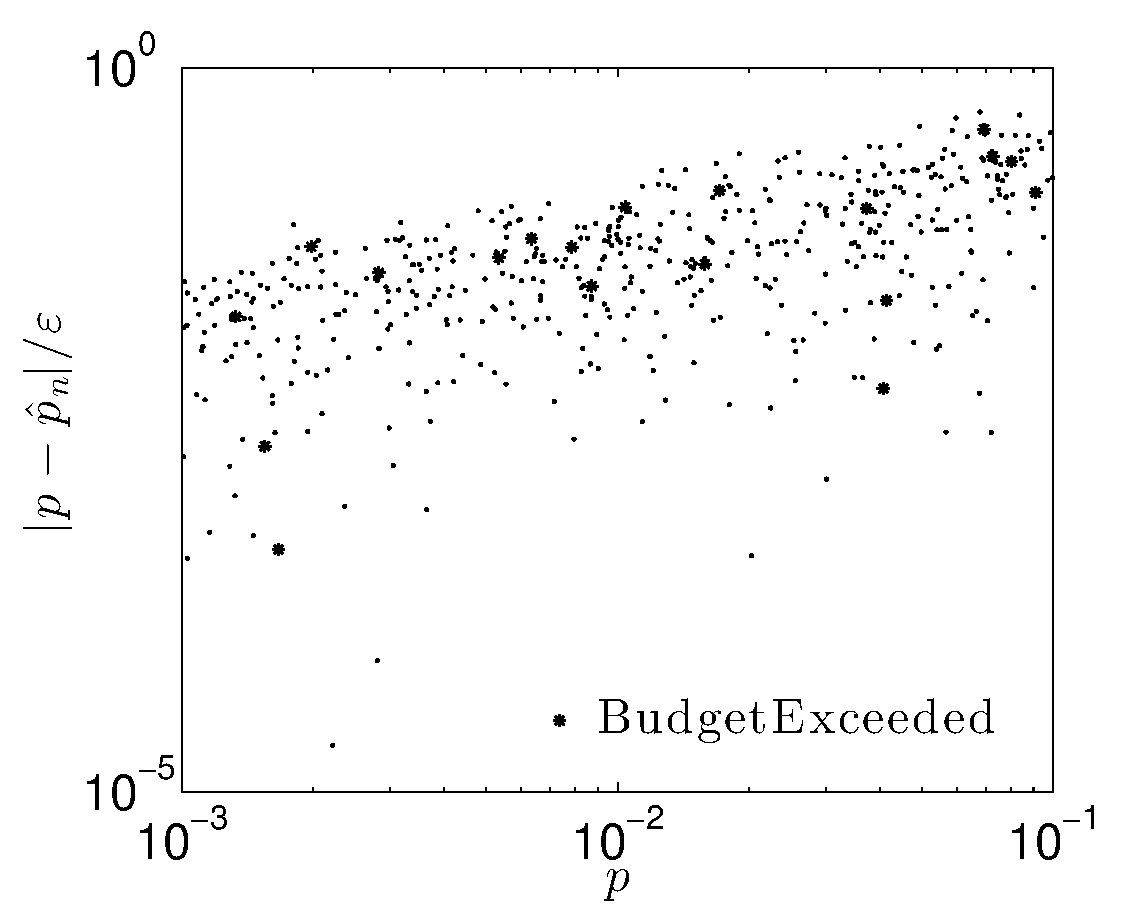
\includegraphics[width=9cm]{abs.eps} % requires the graphicx package
    \caption{Ratio of the actual absolute error to the error tolerance from {\tt meanMCber\_g} versus $p$, for different random samples of $\Ber(p)$ random variables.}
    \label{fig:abserrex}
 \end{figure}
 
While it is encouraging to see that {\tt meanMCber\_g} provides the correct answer in all cases, it is concerning that {\tt meanMCber\_g} is rather conservative for small $p$.  This is due to the fact that the error of $\hp_n$ using $n$ samples is expected to be proportional to $\sqrt{\var(Y)/n}=\sqrt{p(1-p)/n}$.  Even though the error is small for small $p$, our algorithm does not take advantage of that fact.  To do so would require at least a loose lower bound on $p$ at the same time that the algorithm is trying to determine the sample size needed to estimate $p$ carefully.

\Subsection{Test on the relative error criterion}
Another numerical experiment was done with the following parameters:
\begin{itemize}
\item $p$ are given and $\log_{10} p \sim U [-3,-1]$
\item $\varepsilon_r$ are given and random chosen with the distribution $\log_{10} \varepsilon_r \sim U[-2,-1]$
\end{itemize}
  \begin{figure}[htbp]
    \centering
    \includegraphics[width=9cm]{rel.eps} % requires the graphicx package
    \caption{The true relative error/relative error tolerance for different p}
    \label{fig:relerrex}
 \end{figure}
  Similarly, 500 replications were done with random chosen relative error tolerance $\varepsilon_r$ and Bernoulli random variables with random chosen true mean, $p$. In the figure it show that, when $p$ is small, it is more likely to have the sample budget exceeded, as it would be more difficult to estimate the mean with a smaller $p$ than with a larger $p$ with a given relative error tolerance. In more details, we want the condition \eqref{probrel} to be satisfied, there is a denominator which is between $0$ and $1$,  when it gets smaller, we would need a larger sample size to meet this condition.

\Subsection{CLT \& Hoeffding's Inequality Confidence Interval Cost Comparison}
By using Hoeffding's inequality to construct guaranteed fixed-width confidence interval, we definitely incur additional cost compared to an approximate CLT confidence interval.  The ratio of this cost is 
\begin{equation}
\frac{n_{\Hoeff}}{n_{\CLT}} = \frac{\left \lceil \log(2/\alpha)/{2\varepsilon^2} \right \rceil}{\left \lceil{ \Phi^{-1}(1-\alpha/2)}/{4 \varepsilon^2}\right\rceil} \approx  \frac{2\log(2/\alpha)}{\Phi^{-1}(1-\alpha/2)}.
\end{equation}
This ratio essentially depends on the uncertainty level $\alpha$ and is plotted in Figure \ref{fig:ratiovsalpha}. For $\alpha$ between $0.01\%$ to $10\%$ this ratio is between 3.64 to 5.09, which we believe is a reasonable price to pay for the added certainty of {\tt meanMCber\_g}.

  \begin{figure}[htbp]
    \centering
    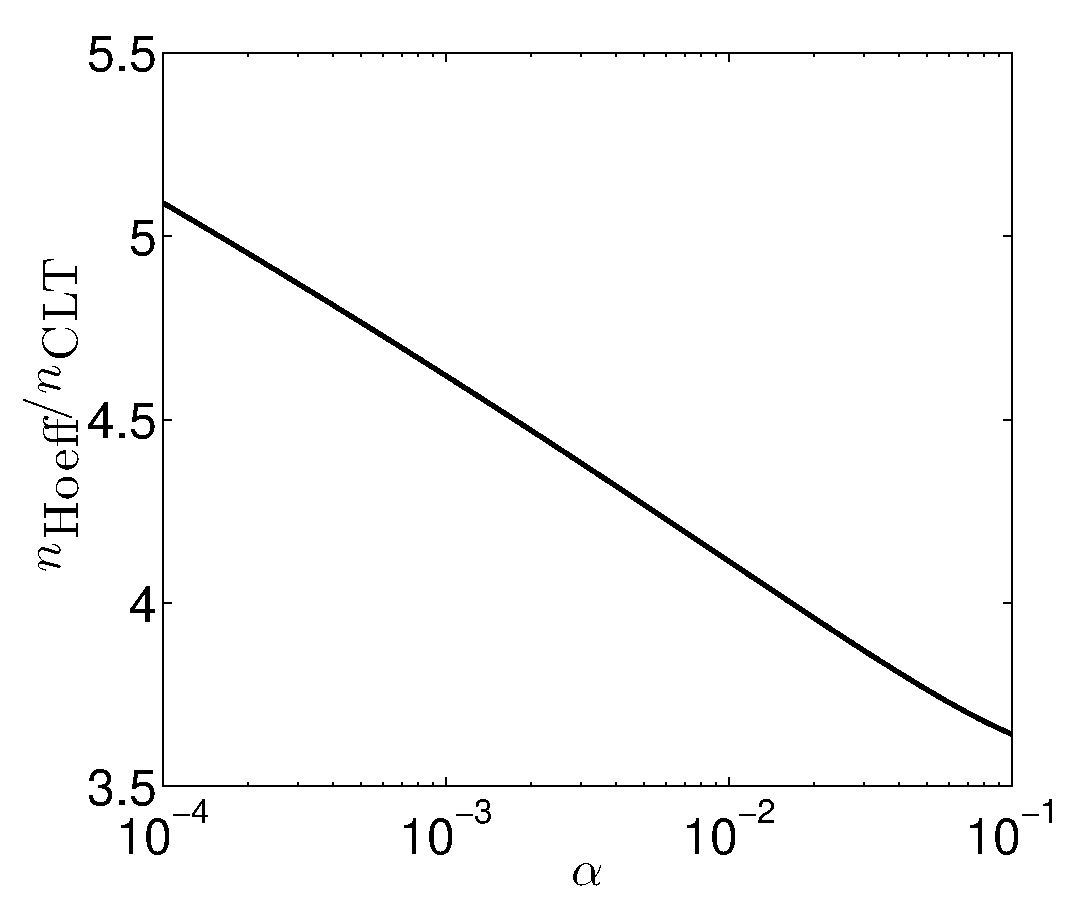
\includegraphics[width=8cm]{plotHoeffCLTr.eps} % requires the graphicx package
    \caption{The computational cost ratio of using Hoeffding's inequality and the CLT to construct a fixed-width confidence interval.}
    \label{fig:ratiovsalpha}
 \end{figure}
 

\Chapter{Conclusion}\label{chapter:comclusion}
\Chapter{Future work}\label{chapter: future work}
We believe that the guaranteed adaptive algorithms are of great interests to the recent practitioners and researchers, as we have suggested a few ways to solve the problems like numerical integration using 1-D trapezoid rule, unit variate function approximation and Monte Carlo methods for evaluating the mean of a random variable,  in \cite{CDHHZ13} and \cite{HJLO12}. Also, we believe these the algorithms followed by theoretical research should be carefully implemented, documented and published, thus, we have been developing our MATLAB toolbox: Guaranteed Automatic Integration Library (GAIL) \cite{GAIL_1_3}. We hope the work in this article will eventually become part of this toolbox.

In this article, the algorithm \ref{algabs} and \ref{algrel} would do the calculation in order to meet either absolute error tolerance or relative error tolerance, another area for further research is to set the tolerance as: $\text{tol} = \max(\varepsilon_a, \varepsilon_r p)$, which may be called as a generalized error tolerance or a hybrid error tolerance. In this way, user would provide both of the tolerance and the algorithm would determine which one would be met first.

As the upper bound of the algorithm \ref{algrel} is given in theorem \ref{costupperboundrel}, the lower bound of the computational complexity is also an area for further research. 

In the paper \cite{HJLO12}, the way to guarantee the absolute error within a prescribed error tolerance has been studied, however, the it is still not clear how to estimate the mean of a random variable to a given relative error tolerance with guarantee. The challenging part is that for relative error, there is a denominator, the probabilistic lower bound of the random variable may be found before we could bound the relative error.
\bibliographystyle{alpha}
\bibliography{Ljiang}
\Appendix{MATLAB Code of meanMCabs\_g}
\lstinputlisting{meanMCabs_g.m}
\Appendix{MATLAB Code of cubMCabs\_g}
\lstinputlisting{cubMCabs_g.m}
\Appendix{MATLAB Code of meanMC\_g}
\lstinputlisting{meanMC_g.m}
%\input{meanMC_g.m}
\Appendix{MATLAB Code of cubMC\_g}
\lstinputlisting{cubMC_g.m}
\Appendix{MATLAB Code of meanMCber\_g}
\lstinputlisting{meanMCber_g.m}

%\input{meanMCgCode}
%\input{cubMCgCode}
%\input{meanMCBergCode}
\end{document}  % end of document